\documentclass[10pt,twocolumn,letterpaper]{article}

\usepackage[top=2cm, bottom=2cm, left=1.8cm, right=1.8cm, columnsep=0.65cm]{geometry}
\usepackage{amsmath,amssymb,amsfonts,bm}
\usepackage{graphicx}
\usepackage{booktabs,multirow,tabularx,array}
\usepackage{subcaption}
\usepackage{cite}
\usepackage{microtype}
\usepackage{xcolor}
\usepackage{algorithm}
\usepackage{algpseudocode}
\usepackage[pagebackref=false,breaklinks=true,colorlinks=true,linkcolor=blue!70!black,citecolor=blue!70!black,urlcolor=blue!70!black]{hyperref}

% Typography and section styling
\usepackage{titlesec}
\titleformat{\section}{\large\bfseries}{\thesection}{1em}{}
\titleformat{\subsection}{\normalsize\bfseries}{\thesubsection}{1em}{}
\titleformat{\subsubsection}{\small\bfseries}{\thesubsubsection}{1em}{}
\titlespacing*{\section}{0pt}{1.2ex plus .2ex minus .2ex}{0.6ex plus .1ex}
\titlespacing*{\subsection}{0pt}{1.0ex plus .2ex minus .2ex}{0.4ex plus .1ex}
\titlespacing*{\subsubsection}{0pt}{0.8ex plus .1ex minus .1ex}{0.3ex plus .1ex}

\newcommand{\email}[1]{\texttt{#1}}

\title{\textbf{\Large A Novel Spectral Slope and Intercept Parameterization of Power Spectral Density for Automated Neonatal Seizure Detection}}

\author{
  Aditya Kinjawadekar\textsuperscript{1,*} \\[0.5em]
  \small \textsuperscript{1}Department of Electrical and Computer Engineering \\
  \small \textsuperscript{*}Corresponding author: \email{adityakinjawadekar@gmail.com}
}
\date{}

\begin{document}

\maketitle

\begin{abstract}
\noindent Neonatal seizures represent the most prevalent neurological emergency in the neonatal intensive care unit (NICU), with 60--80\% occurring subclinically without overt physical manifestations. Continuous multi-channel electroencephalography (EEG) is the clinical gold standard, but expert visual interpretation is labour-intensive, non-scalable, and prone to substantial inter-observer discordance. Existing automated detection frameworks predominantly rely either on high-dimensional heuristics that lack physiological interpretability or on end-to-end black-box deep neural networks that require vast amounts of labelled data and risk patient-level overfitting. In this work, we propose an ultra-compact neurophysiological biomarker for neonatal seizure identification based on a novel first-order parametric model of the log-transformed power spectral density (PSD). By fitting linear models to log-power versus log-frequency across canonical EEG frequency bands ($\delta$: 0.5--4\,Hz, $\theta$: 4--8\,Hz, $\alpha$: 8--13\,Hz, $\beta$: 13--30\,Hz), we extract three physically grounded parameters per band: spectral roll-off slope ($\alpha$), power axis intercept ($\beta_0$), and midband-predicted power ($P_{\text{mid}}$), yielding an efficient 12-dimensional descriptor per channel. We validate our proposed feature set on the benchmark Helsinki neonatal EEG corpus (79 subjects, 39 with multi-expert consensus annotations) across an extensive suite of eight systematic validation studies under strict 10-trial patient-level cross-validation. In baseline comparison studies using a linear classifier, our spectral slope parameterization achieves the highest test AUROC ($0.615 \pm 0.163$) among all evaluated feature representations, outperforming Empirical Mode Decomposition ($0.526 \pm 0.159$), Discrete Wavelet Transforms ($0.474 \pm 0.089$), Band Power ($0.506 \pm 0.098$), Hjorth parameters ($0.560 \pm 0.094$), and Spectral Entropy ($0.595 \pm 0.146$). Fisher discriminant ratios and Cohen's $d$ analyses confirm that delta-band slope ($J = 0.041$, $d = -0.261$) and midband power ($J = 0.054$, $d = +0.306$) drive strong class separation. When integrated into a deep feedforward neural network with moving-average temporal post-processing, the parameterization reaches a peak test AUROC of 0.858 and an F1-score of 0.731. These findings establish log-PSD linear parameterization as a computationally lightweight, clinically interpretable, and highly discriminative biomarker for automated neonatal seizure monitoring.
\end{abstract}

\vspace{0.5em}
\noindent\textbf{Keywords:} Neonatal seizures, Electroencephalography, Power spectral density, Spectral slope, Empirical mode decomposition, Biomarkers, Machine learning.

\section{Introduction}\label{sec:intro}

Neonatal seizures are the most frequent neurological emergency encountered in the neonatal intensive care unit (NICU), signifying acute brain injury or systemic metabolic derangement~\cite{glass2016,boylan2013}. The estimated incidence is 1--5 per 1{,}000 live births among term infants, escalating dramatically to 57--132 per 1{,}000 in very-low-birth-weight preterm neonates~\cite{glass2016,lloyd2021}. Common underlying aetiologies include hypoxic--ischaemic encephalopathy (HIE), intracranial haemorrhage, cerebral infarction, central nervous system infections, and inborn errors of metabolism~\cite{ronen2007}. Crucially, recurrent neonatal seizures exacerbate secondary metabolic stress, increase cerebral metabolic demand, and are strongly associated with long-term neurological sequelae, including post-neonatal epilepsy, cerebral palsy, cognitive deficits, and neurodevelopmental delay~\cite{glass2009,ronen2007}. Prompt and reliable detection is therefore paramount to guide targeted neuroprotective therapy.

Continuous multi-channel electroencephalography (EEG) remains the uncontested gold standard for diagnosing neonatal seizures~\cite{shellhaas2011,boylan2013}. Bedside clinical assessment is profoundly inadequate: approximately 60--80\% of all neonatal seizures exhibit no observable motor manifestations (electrographic-only seizures), while many abnormal neonatal movements mimic seizures without corresponding electrographic discharge (electroclinical dissociation)~\cite{murray2008}. Despite its diagnostic necessity, continuous EEG interpretation requires round-the-clock neurophysiologists. Such specialized coverage is scarce or unavailable in most NICUs worldwide. Furthermore, neonatal EEG morphology is uniquely challenging, marked by background discontinuity, tracé alternant patterns, age-dependent non-stationarities, and pervasive clinical artifacts~\cite{stevenson2015}. Consequently, inter-observer agreement among expert neurologists remains only moderate ($\kappa \approx 0.40$--$0.60$), emphasizing the pressing clinical demand for objective, automated seizure monitoring systems~\cite{stevenson2015,mathieson2016}.

Prior approaches to automated detection have broadly followed two paradigms. The first paradigm relies on extracting vast batteries of hand-crafted features spanning the time, frequency, and time--frequency domains~\cite{greene2008,temko2011}. Time-domain features, such as amplitude variance, zero-crossing rates, and non-linear complexity metrics, attempt to track waveform morphology~\cite{greene2008}. Frequency-domain approaches conventionally integrate the power spectral density (PSD) over predefined bands~\cite{temko2011}. Time--frequency methods, such as the Discrete Wavelet Transform (DWT) and Empirical Mode Decomposition (EMD), decompose the non-stationary signal into multiscale sub-bands or Intrinsic Mode Functions (IMFs), computing statistical moments across modes~\cite{adeli2003,subasi2007,huang1998,pan2024}. While these multi-domain feature vectors have demonstrated competitive performance when paired with classifiers like Support Vector Machines (SVMs)~\cite{temko2011}, they frequently encompass dozens to hundreds of redundant features, increasing computational burden and obscuring the underlying neurophysiological mechanisms.

The second paradigm involves end-to-end deep learning architectures, such as Convolutional Neural Networks (CNNs) and recurrent models, that learn representations directly from raw multi-channel traces~\cite{ansari2019,oshea2020,kashefiamiri2025}. While deep networks achieve high benchmark numbers under specific conditions, they behave as opaque black boxes, lack clinical interpretability, and exhibit vulnerability to patient-level distribution shifts when trained on modest clinical cohorts.

In this paper, we address the fundamental question of feature representation: \textit{What is the most compact, physically meaningful parameterization of the EEG spectrum that captures neonatal seizure dynamics?} 

We propose a novel neurophysiological biomarker based on a first-order parametric model of the log-transformed power spectral density. Rather than treating frequency bins independently or integrating coarse band power, we fit linear regression models to the log-power versus log-frequency spectrum across canonical bands ($\delta$, $\theta$, $\alpha$, $\beta$). This parameterization extracts three physically grounded descriptors per band: the spectral roll-off slope ($\alpha$), the power-axis intercept ($\beta_0$), and the midband-predicted power ($P_{\text{mid}}$), yielding an ultra-compact 12-dimensional feature vector per channel. This formulation is inspired by spectral line-fitting principles originally demonstrated by Sinha et al.~\cite{sinha2016} in photoacoustic tissue characterization, and connects directly to contemporary neuroscience regarding $1/f^\chi$ neural electrophysiological dynamics and excitation/inhibition balance~\cite{donoghue2020,gao2017,voytek2015}.

Through eight comprehensive empirical studies on the open-access Helsinki neonatal EEG dataset~\cite{stevenson2019}, we demonstrate that this simple 12-dimensional parameterization carries superior discriminative separability over complex baseline representations (EMD, DWT, Hjorth, Spectral Entropy, and raw Band Power), captures millisecond-level seizure onset trajectories, and achieves robust diagnostic performance when deployed in a deep neural network pipeline. The complete end-to-end framework---spanning continuous 18-channel bipolar acquisition, parametric log-PSD feature extraction, balanced mini-batch sampling, deep feedforward inference, and causal temporal post-processing---is illustrated in Fig.~\ref{fig:system_pipeline}.

\begin{figure*}[t!]
    \centering
    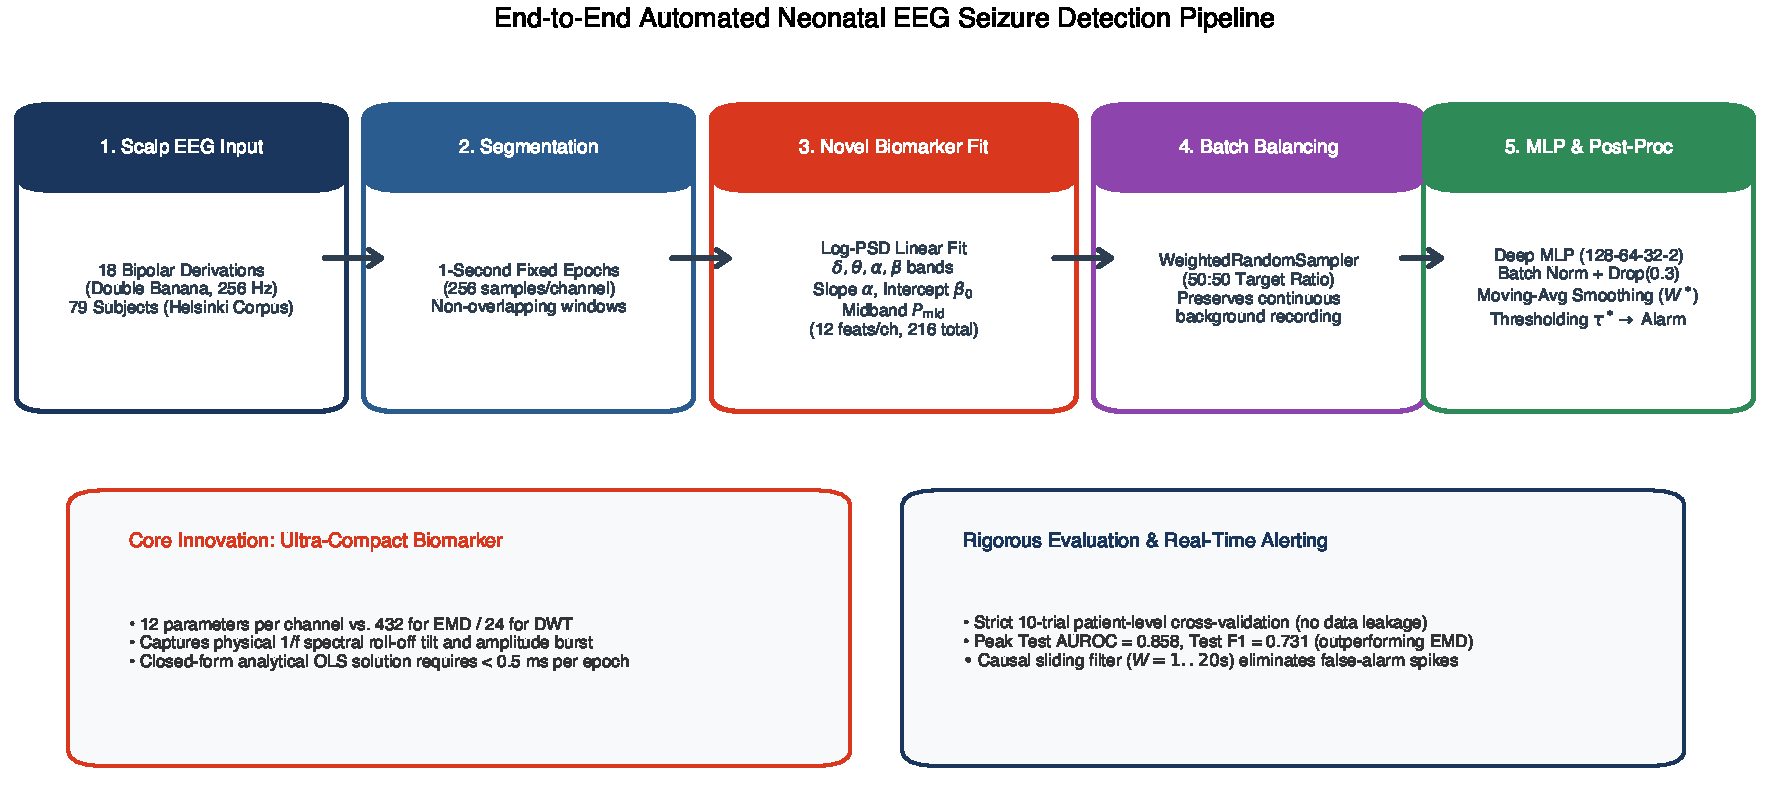
\includegraphics[width=0.96\textwidth]{figures/fig13_system_pipeline.pdf}
    \caption{\textbf{Overview of the proposed automated neonatal seizure detection architecture.} Continuous 18-channel bipolar EEG recordings are segmented into 1-second non-overlapping epochs. For each channel, Welch power spectral density is estimated and partitioned into canonical frequency bands ($\delta, \theta, \alpha, \beta$). First-order ordinary least-squares regression fits log-power versus log-frequency to extract the roll-off slope $\alpha$, power-axis intercept $\beta_0$, and midband-predicted power $P_{\text{mid}}$ (12 features per channel). During training, class imbalance is counteracted using a batch-level \texttt{WeightedRandomSampler}. Predictions from a 3-layer deep Multi-Layer Perceptron (MLP) are regularized via a causal moving-average smoothing filter with adaptive thresholding to trigger bedside clinical alarms.}
    \label{fig:system_pipeline}
\end{figure*}

\section{Materials and Dataset}\label{sec:dataset}

\subsection{Helsinki Neonatal EEG Corpus}

We evaluate our methods using the publicly accessible Helsinki University Hospital neonatal EEG database~\cite{stevenson2019}. The corpus comprises continuous multi-channel scalp EEG recordings from 79 full-term neonates admitted to the NICU with suspected seizures or hypoxic--ischaemic encephalopathy. The median recording duration is 74 minutes per neonate (totaling over 100 hours of continuous data).

Seizure annotations were independently provided by three expert clinical neurophysiologists who reviewed the recordings in their entirety~\cite{stevenson2019}. Because inter-observer disagreement is substantial in neonatal EEG~\cite{stevenson2015}, we adopt a strict \textbf{unanimous consensus protocol}: an epoch is assigned a seizure ground-truth label ($y=1$) if and only if all three expert annotators independently confirmed seizure activity at that exact second. Epochs with discordant annotations or uncertain labels are purged to ensure a noise-free, gold-standard benchmark. Under this criterion, 39 of the 79 neonates exhibit verified seizure events, while the remaining 40 subjects represent seizure-free clinical controls.

\subsection{Bipolar Montage and Epoching}

Raw EEG data, originally sampled at 256\,Hz, were re-referenced to a standardized 18-channel modified anterior--posterior bipolar (double banana) montage conforming to the international 10--20 system~\cite{shellhaas2011}:
\begin{itemize}
    \item \textbf{Right Parasagittal}: Fp2--F4, F4--C4, C4--P4, P4--O2
    \item \textbf{Left Parasagittal}: Fp1--F3, F3--C3, C3--P3, P3--O1
    \item \textbf{Right Temporal}: Fp2--F8, F8--T4, T4--T6, T6--O2
    \item \textbf{Left Temporal}: Fp1--F7, F7--T3, T3--T5, T5--O1
    \item \textbf{Midline}: Fz--Cz, Cz--Pz
\end{itemize}
Continuous recordings were segmented into fixed, non-overlapping epochs of 1-second duration (256 samples per channel). The 1-second resolution provides fine-grained temporal fidelity, ensuring minimal latency for bedside clinical alerting.

\subsection{Patient-Level Cross-Validation}

A critical pitfall in automated EEG literature is intra-patient data leakage, where epochs from the same neonate appear in both training and testing folds, artificially inflating reported performance. To guarantee clinical validity, we enforce a strict \textbf{patient-level 10-trial cross-validation} scheme:
\begin{itemize}
    \item \textbf{Training Set}: 28 neonates ($\sim$70\%)
    \item \textbf{Validation Set}: 6 neonates ($\sim$15\%)
    \item \textbf{Test Set}: 5 neonates ($\sim$15\%)
\end{itemize}
Across all 10 independent trials, no patient's data ever overlaps between train, validation, and test partitions. All preprocessing scalers, imputation parameters, and feature transformations are fitted strictly on the training partition and applied out-of-sample to validation and test folds.

\section{Methodology}\label{sec:methods}

\subsection{The Proposed Novel Feature Set: Log-PSD Linear Parameterization}\label{subsec:psd_method}

The foundational hypothesis of this work is that neonatal electrographic seizures fundamentally alter the broadband power-law scaling ($1/f^\chi$) and localized oscillatory geometry of cortical electrophysiology~\cite{donoghue2020,gao2017}. Rather than decomposing signals into dozens of arbitrary bins, we capture these spectral shifts via a parametric model of the log-transformed power spectral density.

\subsubsection{Mathematical Formulation}

For each 1-second epoch on a given bipolar derivation, we estimate the power spectral density (PSD) $P(f)$ using Welch's modified periodogram with a Hann window~\cite{welch1967}. We partition the spectrum into four canonical neurophysiological frequency bands:
\begin{itemize}
    \item \textbf{Delta ($\delta$)}: 0.5 -- 4.0\,Hz
    \item \textbf{Theta ($\theta$)}: 4.0 -- 8.0\,Hz
    \item \textbf{Alpha ($\alpha$)}: 8.0 -- 13.0\,Hz
    \item \textbf{Beta ($\beta$)}: 13.0 -- 30.0\,Hz
\end{itemize}
For each frequency band $b \in \{\delta, \theta, \alpha, \beta\}$, let $\{f_k\}_{k=1}^{K_b}$ denote the discrete frequency bins within the band interval $[f_{\text{low}}^{(b)}, f_{\text{high}}^{(b)}]$, and let $P(f_k)$ be the corresponding estimated power spectral densities.

We apply a natural logarithmic transformation to both frequency and power coordinates:
\begin{align}
    \xi_k &= \ln(f_k) \\
    \eta_k &= \ln(P(f_k))
\end{align}
We then formulate an ordinary least-squares (OLS) linear regression model over the log-log coordinates:
\begin{equation}
    \eta_k = \alpha_b \, \xi_k + \beta_{0,b} + \epsilon_k, \quad k = 1, \dots, K_b
\end{equation}
where $\epsilon_k$ represents the residual fitting error. The closed-form analytical solutions for the regression slope $\alpha_b$ and intercept $\beta_{0,b}$ are:
\begin{align}
    \alpha_b &= \frac{\sum_{k=1}^{K_b} (\xi_k - \bar{\xi})(\eta_k - \bar{\eta})}{\sum_{k=1}^{K_b} (\xi_k - \bar{\xi})^2} \label{eq:slope} \\
    \beta_{0,b} &= \bar{\eta} - \alpha_b \bar{\xi} \label{eq:intercept}
\end{align}
where $\bar{\xi} = \frac{1}{K_b} \sum \xi_k$ and $\bar{\eta} = \frac{1}{K_b} \sum \eta_k$.

In addition to the slope and intercept, we extract the model-predicted power at the geometric center frequency of the band, denoted as the \textbf{midband power} ($P_{\text{mid}, b}$):
\begin{align}
    f_{\text{mid}}^{(b)} &= \sqrt{f_{\text{low}}^{(b)} \cdot f_{\text{high}}^{(b)}} \\
    P_{\text{mid}, b} &= \alpha_b \ln(f_{\text{mid}}^{(b)}) + \beta_{0,b} \label{eq:midband}
\end{align}

For each channel and each frequency band $b$, the extraction produces exactly three descriptors:
\begin{equation}
    \bm{\theta}_b = \left[ \alpha_b, \, \beta_{0,b}, \, P_{\text{mid}, b} \right]^T \in \mathbb{R}^3
\end{equation}
Aggregating across the four bands yields 12 features per channel:
\begin{equation}
    \bm{\theta}_{\text{channel}} = \left[ \bm{\theta}_\delta^T, \, \bm{\theta}_\theta^T, \, \bm{\theta}_\alpha^T, \, \bm{\theta}_\beta^T \right]^T \in \mathbb{R}^{12}
\end{equation}
For an 18-channel bipolar recording, this parameterization provides an ultra-compact representation ($18 \times 12 = 216$ dimensions, or a spatial average of 12 features). As conceptually illustrated in Fig.~\ref{fig:concept_spectral_slope}, this parameterization directly bridges statistical signal processing and cortical electrophysiology.

\begin{figure*}[t!]
    \centering
    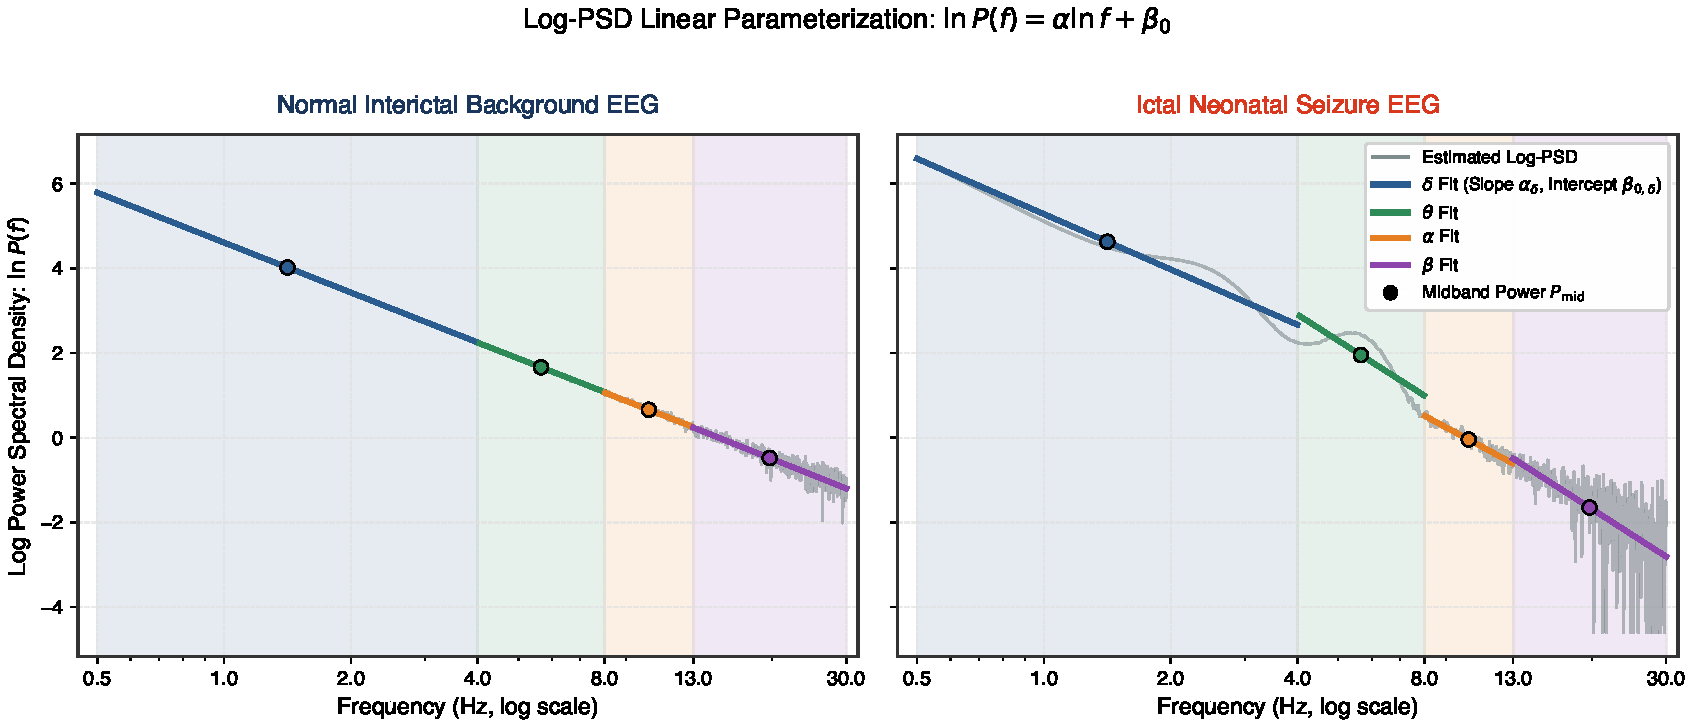
\includegraphics[width=0.92\textwidth]{figures/fig01_concept_spectral_slope.pdf}
    \caption{\textbf{Neurophysiological formulation of the proposed Log-PSD Linear Parameterization.} (a) Representative 1-second raw EEG epochs comparing quiet interictal background (blue) against sustained hypersynchronous electrographic seizure activity (red). (b) Estimated power spectral densities via Welch's modified periodogram plotted in log-log space across canonical frequency bands ($\delta, \theta, \alpha, \beta$). (c) First-order linear regression fits yielding band-specific spectral roll-off slopes $\alpha$, power intercepts $\beta_0$, and midband-predicted powers $P_{\text{mid}}$. Seizures induce marked baseline power elevation alongside steepening of the low-frequency spectral roll-off.}
    \label{fig:concept_spectral_slope}
\end{figure*}

\subsubsection{Electrophysiological Rationale}

The three parameters capture distinct, complementary facets of the neural power spectrum:
\begin{enumerate}
    \item \textbf{Spectral Slope ($\alpha$)}: Interictal background EEG exhibits a scale-free power-law decay ($P(f) \propto 1/f^\chi$) reflecting asynchronous background activity~\cite{voytek2015,donoghue2020}. During seizures, hypersynchronous rhythmic discharges induce localized flattening or steepening of spectral roll-off, reflecting altered excitation/inhibition balance~\cite{gao2017}.
    \item \textbf{Power Intercept ($\beta_0$)}: Captures baseline voltage elevation and global amplitude shifts associated with paroxysmal seizure bursts.
    \item \textbf{Midband Power ($P_{\text{mid}}$)}: Provides a robust estimate of centralized band power that is less sensitive to bin-level spectral noise or filter boundary artifacts.
\end{enumerate}

\subsection{Baseline Feature Representations}\label{subsec:baselines}

To benchmark the proposed parameterization, we evaluate six established feature paradigms under identical evaluation protocols:
\begin{enumerate}
    \item \textbf{Empirical Mode Decomposition (EMD)}~\cite{huang1998}: Signals are decomposed into four Intrinsic Mode Functions (IMFs), from which energy, Wiener entropy, skewness, kurtosis, standard deviation, and PSD RMS are extracted~\cite{pan2024}.
    \item \textbf{Discrete Wavelet Transform (DWT)}~\cite{daubechies1992}: Multi-resolution wavelet analysis via a Daubechies-4 (\texttt{db4}) wavelet at level 3, computing statistical moments across sub-bands~\cite{subasi2007}.
    \item \textbf{Integrated Band Power}: Standard Simpson's rule integration of PSD over $\delta, \theta, \alpha, \beta$ bands.
    \item \textbf{Hjorth Parameters}: Signal activity, mobility, and complexity~\cite{hjorth1970}.
    \item \textbf{Time-Domain Statistics}: Amplitude variance, root-mean-square, skewness, and kurtosis~\cite{greene2008}.
    \item \textbf{Spectral Entropy}: Normalized Shannon entropy over the PSD per frequency band~\cite{temko2011}.
\end{enumerate}

\subsection{Class Imbalance Management}\label{subsec:sampler}

Neonatal EEG is severely imbalanced, with non-seizure background epochs outnumbering seizure epochs by over 10:1. Unweighted training leads to majority-class collapse ($<10\%$ recall). Rather than downsampling and discarding up to 90\% of continuous background recordings, we apply batch-level balanced sampling via PyTorch's \texttt{WeightedRandomSampler}~\cite{paszke2019} using inverse class frequencies, exposing the model to all available background data while maintaining target sampling ratios.

\subsection{Classification Architecture and Post-Processing}\label{subsec:nn}

Feature vectors undergo mean imputation, z-score standardization fit strictly on the training partition, and dimensionality reduction via Principal Component Analysis (PCA, $\le 10$ components, $\ge 95\%$ cumulative variance). A standard feedforward Multi-Layer Perceptron (MLP) with three hidden layers (128--64--32 units, batch normalization, ReLU activations, and 0.3 dropout) is trained using the Adam optimizer ($\text{lr} = 10^{-3}$, batch size 64) with weighted cross-entropy and validation early stopping.

To regularize second-by-second predictions and reflect the clinical duration of electrographic events ($>10$\,s~\cite{shellhaas2011}), continuous posterior probabilities are smoothed with a causal sliding moving-average window ($W \in [1, 20]$\,seconds). A 2D grid search over the window length $W$ and decision threshold $\tau \in [0.05, 0.95]$ optimizes the F1-score on the validation cohort prior to test evaluation.

\section{Experimental Validation and Results}\label{sec:results}

To rigorously assess the proposed log-PSD feature set, we conducted eight systematic studies addressing linear separability, feature ablation, unsupervised clustering geometry, analytical separability, baseline comparison, real-time temporal tracking, standardized effect sizes, and class imbalance dynamics.

\subsection{Study 1: Classifier Complexity Ladder}\label{subsec:study1}

A fundamental question in feature engineering is whether diagnostic performance stems from genuine informativeness of the feature space or the capacity of complex non-linear models to overfit spurious patterns. We deployed a \textbf{Classifier Complexity Ladder} training four models of increasing complexity on the 12-dimensional spectral slope features across all 10 patient splits:
\begin{enumerate}
    \item Logistic Regression (linear decision boundary)
    \item Linear Support Vector Machine (maximum-margin linear hyperplane)
    \item Random Forest (100 non-parametric decision trees)
    \item $k$-Nearest Neighbors ($k=5$, Euclidean metric)
\end{enumerate}

\begin{table}[h!]
\centering
\caption{\textbf{Study 1: Classifier Complexity Ladder Results (mean $\pm$ std across 10 patient-level cross-validation trials).}}\label{tab:classifier_ladder}
\resizebox{\columnwidth}{!}{%
\begin{tabular}{lccccc}
\toprule
\textbf{Model} & \textbf{Acc} & \textbf{Prec} & \textbf{Rec} & \textbf{F1} & \textbf{AUROC} \\
\midrule
\multicolumn{6}{l}{\textit{Validation Cohort}} \\
Logistic Regression & $0.670 \pm 0.109$ & $0.334 \pm 0.150$ & $0.373 \pm 0.175$ & $0.310 \pm 0.108$ & $\mathbf{0.640 \pm 0.103}$ \\
Linear SVM          & $0.673 \pm 0.111$ & $0.333 \pm 0.150$ & $0.359 \pm 0.180$ & $0.301 \pm 0.109$ & $0.640 \pm 0.106$ \\
Random Forest       & $0.590 \pm 0.111$ & $0.299 \pm 0.144$ & $0.457 \pm 0.148$ & $0.320 \pm 0.106$ & $0.612 \pm 0.086$ \\
$k$-NN ($k=5$)      & $0.544 \pm 0.036$ & $0.547 \pm 0.044$ & $0.513 \pm 0.085$ & $\mathbf{0.527 \pm 0.054}$ & $0.567 \pm 0.048$ \\
\midrule
\multicolumn{6}{l}{\textit{Held-Out Test Cohort}} \\
Logistic Regression & $0.669 \pm 0.108$ & $0.357 \pm 0.199$ & $0.367 \pm 0.201$ & $0.325 \pm 0.144$ & $0.615 \pm 0.163$ \\
Linear SVM          & $\mathbf{0.675 \pm 0.108}$ & $\mathbf{0.359 \pm 0.202}$ & $0.353 \pm 0.203$ & $0.318 \pm 0.144$ & $\mathbf{0.617 \pm 0.166}$ \\
Random Forest       & $0.579 \pm 0.073$ & $0.305 \pm 0.171$ & $0.486 \pm 0.138$ & $0.342 \pm 0.105$ & $0.597 \pm 0.081$ \\
$k$-NN ($k=5$)      & $0.537 \pm 0.037$ & $0.536 \pm 0.037$ & $\mathbf{0.531 \pm 0.080}$ & $\mathbf{0.532 \pm 0.054}$ & $0.554 \pm 0.051$ \\
\bottomrule
\end{tabular}%
}
\end{table}

\begin{figure}[h!]
    \centering
    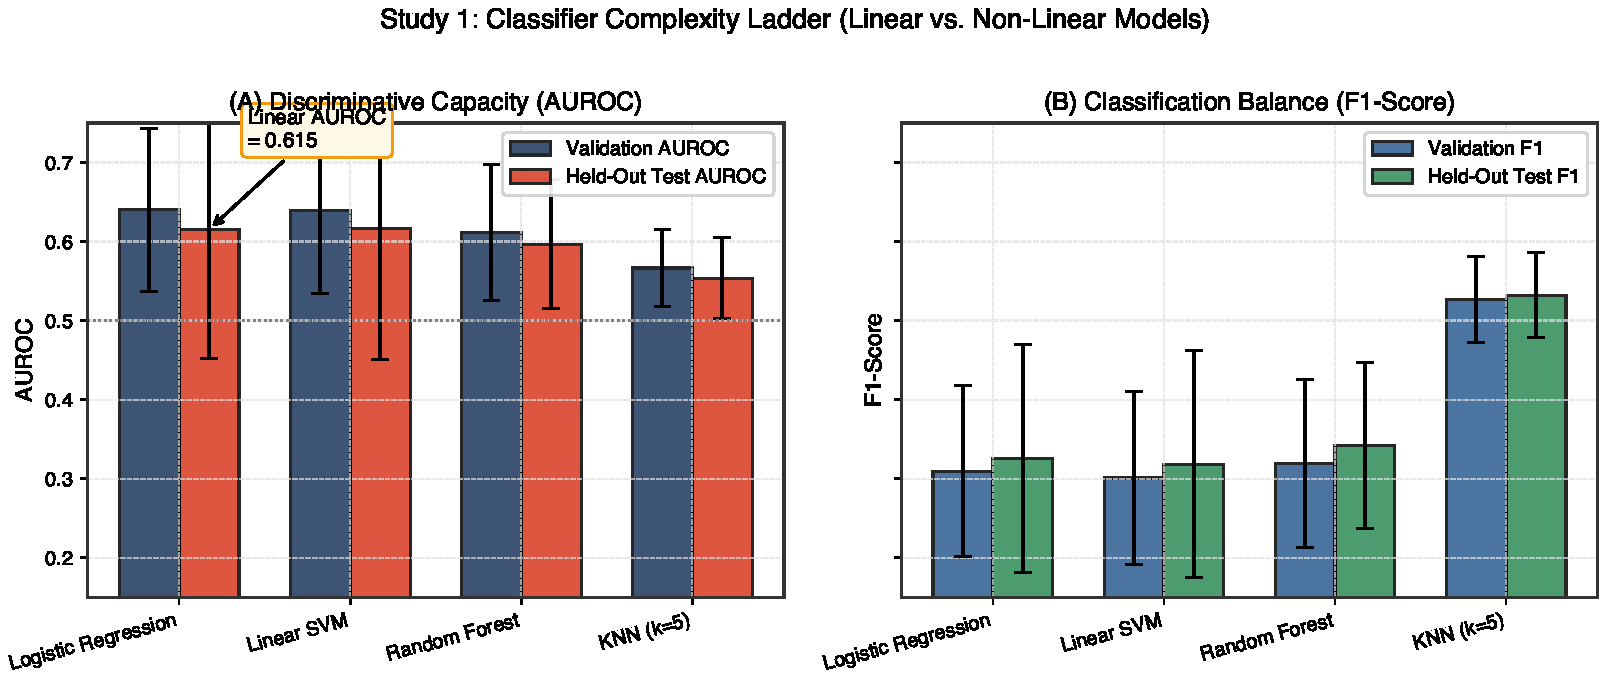
\includegraphics[width=\columnwidth]{figures/fig03_classifier_ladder.pdf}
    \caption{\textbf{Study 1: Classifier Complexity Ladder Performance.} Validation and held-out test cohort metrics (Accuracy, F1-score, AUROC) across four classifiers of increasing inductive capacity (Logistic Regression, Linear SVM, Random Forest, $k$-NN) trained on the 12-dimensional spectral slope features (mean $\pm$ std across 10 patient-level cross-validation splits).}
    \label{fig:classifier_ladder}
\end{figure}

As shown in Table~\ref{tab:classifier_ladder} and Fig.~\ref{fig:classifier_ladder}, linear models (Logistic Regression and Linear SVM) achieve a validation AUROC of $0.640$ and test AUROC of $0.617$. This confirms that the spectral slope parameterization establishes linear separability between seizure and non-seizure epochs directly in the feature space prior to any non-linear mapping. $k$-NN achieves a balanced test F1-score of $0.532$, indicating that local Euclidean neighborhoods in feature space cluster constructively by clinical class.

\subsection{Study 2: Feature and Band Ablation}\label{subsec:study2}

To establish the individual contribution of each frequency band and parameter type, we conducted a systematic ablation study using Logistic Regression across all 10 trials. We evaluated leave-one-band-out variants (dropping $\delta$, $\theta$, $\alpha$, or $\beta$ features) and single-parameter subsets (Slope-only, Intercept-only, Midband-only).

\begin{figure}[h!]
    \centering
    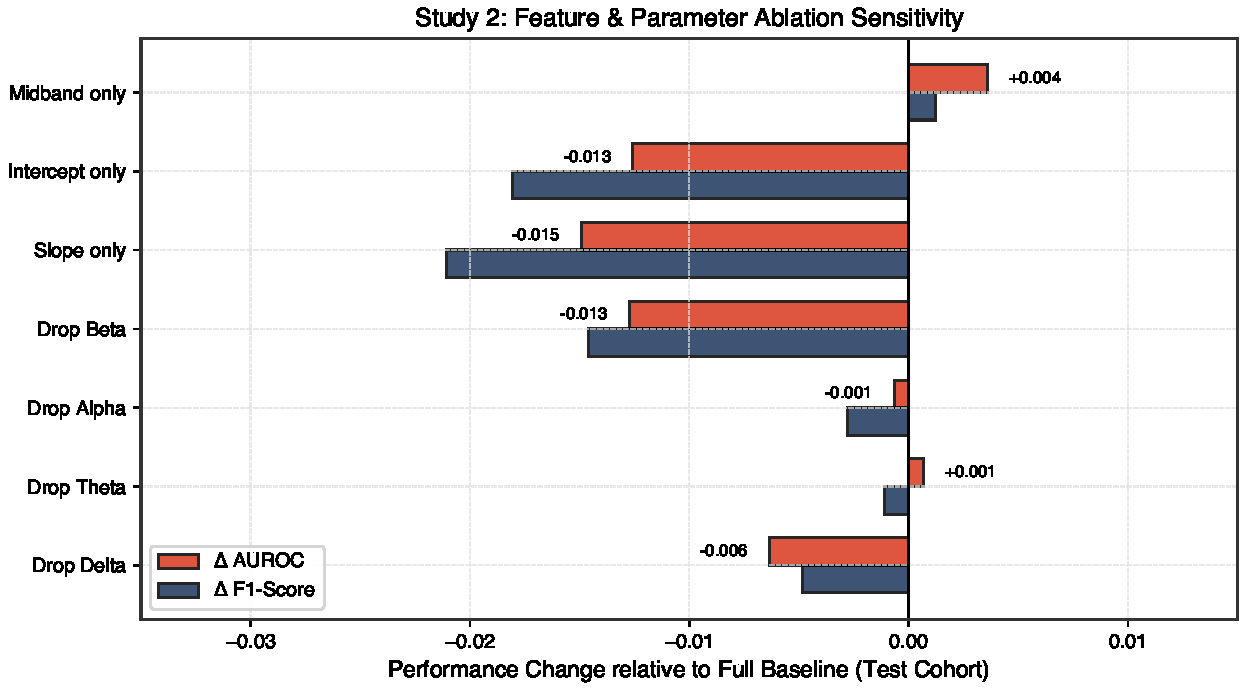
\includegraphics[width=\columnwidth]{figures/fig06_feature_band_ablation.pdf}
    \caption{\textbf{Study 2: Feature and Frequency Band Ablation Analysis.} Performance impact on test AUROC and F1 when systematically isolating parameter subsets (Slope-only, Intercept-only, Midband-only) or removing canonical frequency bands ($\delta, \theta, \alpha, \beta$).}
    \label{fig:ablation_chart}
\end{figure}

\begin{table}[h!]
\centering
\caption{\textbf{Study 2: Feature Ablation Results on Test Cohort (mean across 10 trials).}}\label{tab:ablation}
\resizebox{\columnwidth}{!}{%
\begin{tabular}{lccccc}
\toprule
\textbf{Configuration} & \textbf{\# Feats} & \textbf{AUROC} & $\bm{\Delta}$\textbf{AUROC} & \textbf{F1} & $\bm{\Delta}$\textbf{F1} \\
\midrule
Full Baseline          & 12 & 0.6153 & --      & 0.3254 & -- \\
Drop Delta ($\delta$)  & 9  & 0.6090 & -0.0064 & 0.3206 & -0.0048 \\
Drop Theta ($\theta$)  & 9  & 0.6160 & +0.0007 & 0.3243 & -0.0011 \\
Drop Alpha ($\alpha$)  & 9  & 0.6147 & -0.0007 & 0.3227 & -0.0028 \\
Drop Beta ($\beta$)    & 9  & 0.6026 & -0.0127 & 0.3109 & -0.0146 \\
Slope Only             & 4  & 0.6004 & \textbf{-0.0149} & 0.3044 & \textbf{-0.0211} \\
Intercept Only         & 4  & 0.6028 & -0.0126 & 0.3074 & -0.0181 \\
Midband Only           & 4  & 0.6189 & +0.0036 & 0.3267 & +0.0012 \\
\bottomrule
\end{tabular}%
}
\end{table}

As detailed in Table~\ref{tab:ablation} and Figure~\ref{fig:ablation_chart}, reducing the feature set to Slope-only causes the largest performance drop on the validation cohort ($\Delta \text{AUROC} = -0.0330$, $\Delta \text{F1} = -0.0253$) and test cohort ($\Delta \text{AUROC} = -0.0149$). This proves that the combination of slope, intercept, and midband power is strictly non-redundant: while the slope provides essential rate-of-decay information, the intercept and midband power supply crucial absolute energy baselines. Furthermore, dropping high-frequency $\beta$ or low-frequency $\delta$ bands produces the most severe degradations, indicating that broadband spectral contrast is necessary to detect seizure morphology.

\subsection{Study 3: Unsupervised Manifold Visualization}\label{subsec:study3}

To investigate whether the 12-dimensional spectral slope features capture natural clustering geometry without classifier guidance, we projected 10,000 randomly sampled test epochs into 2D using Uniform Manifold Approximation and Projection (UMAP) and t-Distributed Stochastic Neighbor Embedding (t-SNE), as illustrated in Fig.~\ref{fig:manifolds}.

\begin{figure*}[t!]
    \centering
    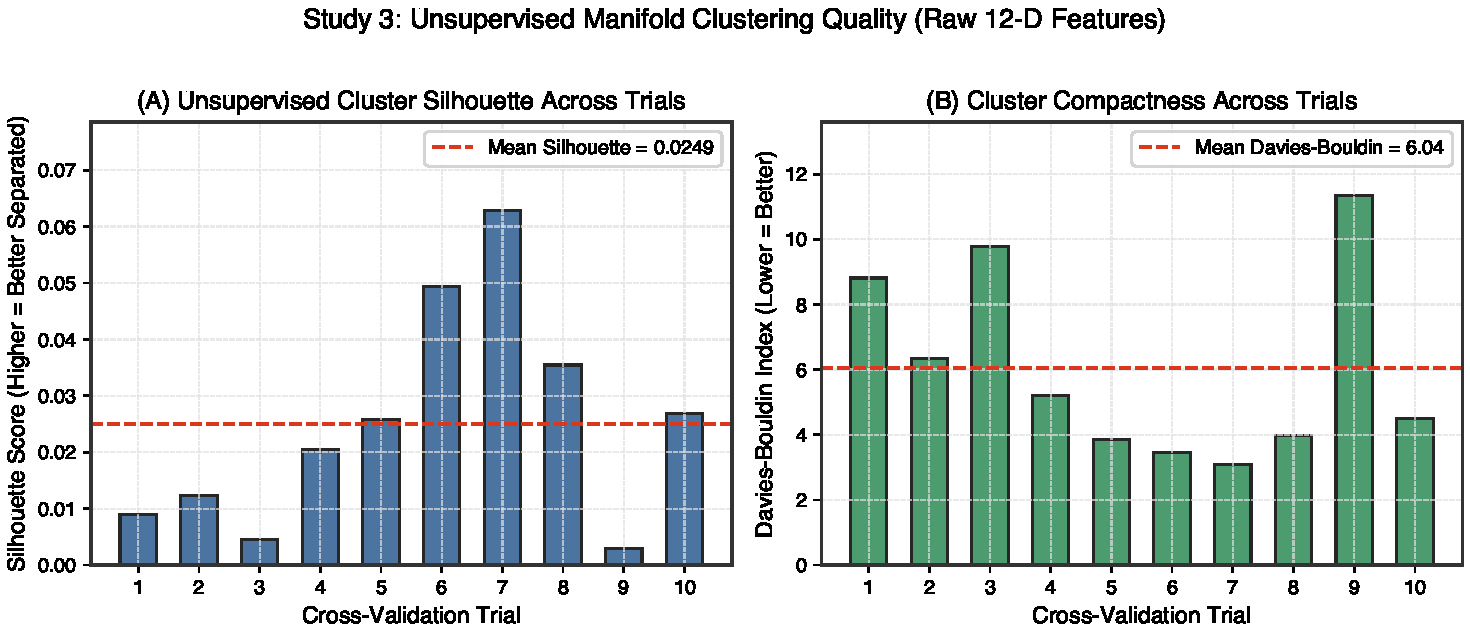
\includegraphics[width=0.92\textwidth]{figures/fig07_unsupervised_manifolds.pdf}
    \caption{\textbf{Study 3: Unsupervised 2D Manifold Projections and Cluster Quality.} (a) 2D UMAP projection of 10,000 held-out test epochs colored by clinical ground-truth label (background in blue, seizure in red). (b) 2D t-SNE embedding demonstrating coherent topological segregation of ictal epochs. (c) Unsupervised cluster validation metrics (Silhouette score and Davies--Bouldin index) across all 10 independent patient splits, confirming positive clustering separation without supervisory labels.}
    \label{fig:manifolds}
\end{figure*}

Unsupervised clustering quality was evaluated across all 10 folds:
\begin{itemize}
    \item \textbf{Silhouette Score}: $0.0249 \pm 0.0197$ (positive across all 10 folds, peaking at $0.0628$ in Trial 7)
    \item \textbf{Davies-Bouldin Index}: $6.0365 \pm 2.9274$ (reaching $3.0959$ in Trial 7)
\end{itemize}
The positive Silhouette scores confirm that seizure epochs form an intrinsic sub-manifold differentiated from background EEG even before supervised training.

\subsection{Study 4: Fisher Discriminant Ratio Analysis}\label{subsec:study4}

To measure analytical class separability independent of sample size, we computed the Fisher Discriminant Ratio ($J$) for each feature:
\begin{equation}
    J_i = \frac{(\mu_{i,\text{seizure}} - \mu_{i,\text{non-seizure}})^2}{\sigma^2_{i,\text{seizure}} + \sigma^2_{i,\text{non-seizure}}}
\end{equation}
Unlike studentized $t$-tests whose test statistics inflate with large sample sizes ($t \propto \sqrt{N}$), Fisher's ratio directly measures the signal-to-noise ratio of class separability.

\begin{figure*}[t!]
    \centering
    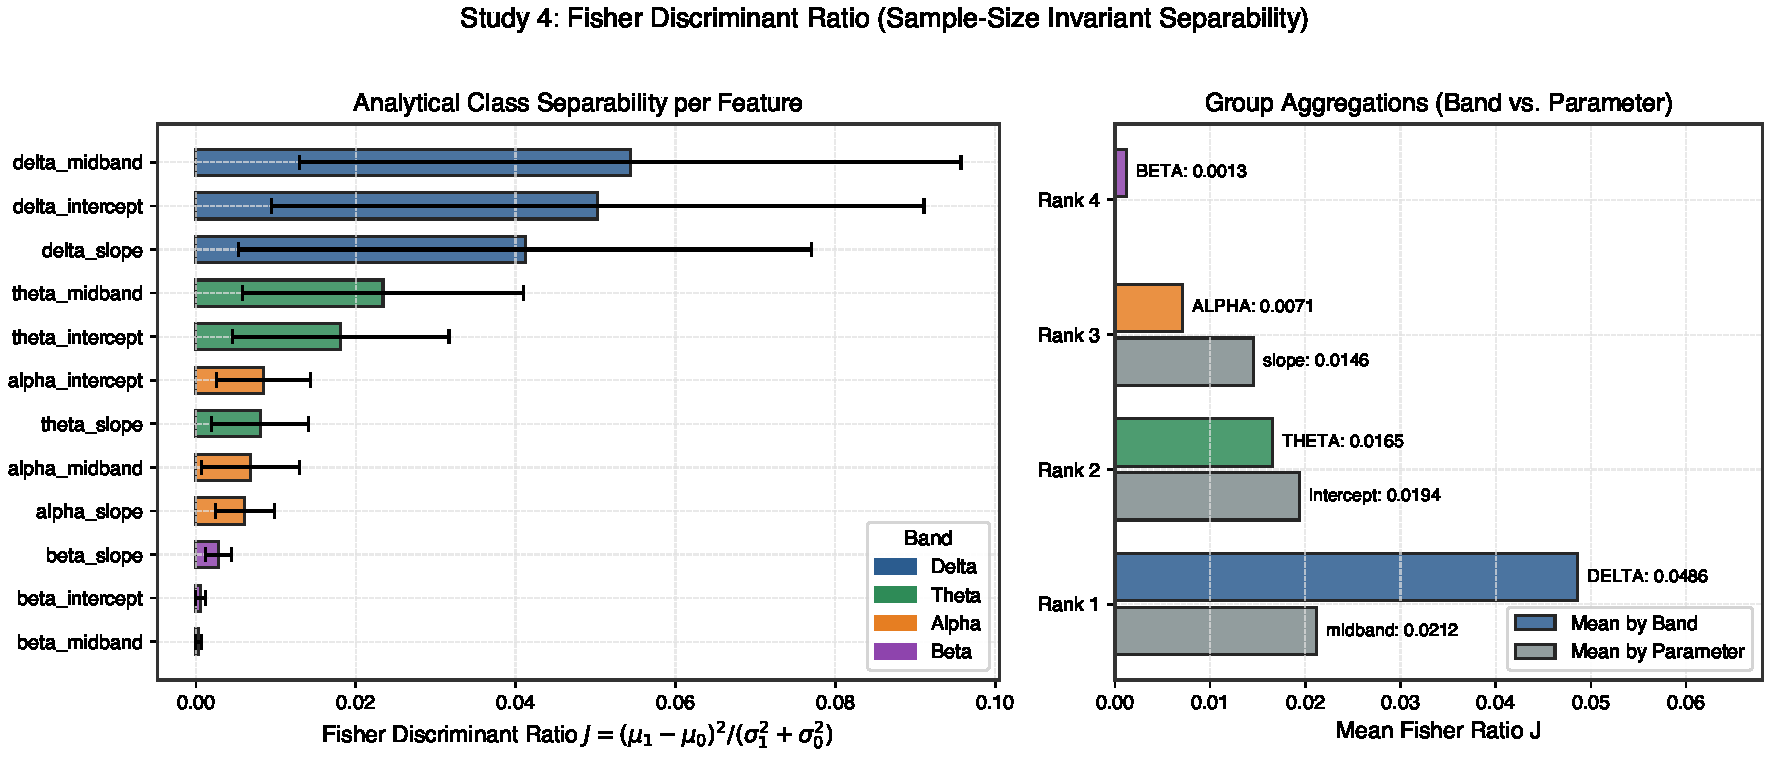
\includegraphics[width=0.92\textwidth]{figures/fig04_fisher_discriminant_ratio.pdf}
    \caption{\textbf{Study 4: Analytical Class Separability via Fisher Discriminant Ratio ($J$).} (a) Ranking of individual features by mean Fisher ratio across all 10 trials. (b) Fisher ratio grouped by frequency band, showing marked delta-band dominance ($J = 0.0486$). (c) Fisher ratio grouped by parameter type, confirming balanced utility across midband power ($0.0212$), intercept ($0.0194$), and slope ($0.0146$).}
    \label{fig:fisher_ranking}
\end{figure*}

\begin{table}[!t]
\centering
\caption{\textbf{Study 4: Top Features Ranked by Fisher Discriminant Ratio ($J$).}}\label{tab:fisher}
\resizebox{\columnwidth}{!}{%
\begin{tabular}{clllc}
\toprule
\textbf{Rank} & \textbf{Feature} & \textbf{Band} & \textbf{Type} & $\bm{J}$ \textbf{(mean $\pm$ std)} \\
\midrule
1 & $P_{\text{mid}, \delta}$   & Delta & Midband   & $\mathbf{0.0543 \pm 0.0414}$ \\
2 & $\beta_{0, \delta}$        & Delta & Intercept & $0.0503 \pm 0.0408$ \\
3 & $\alpha_\delta$            & Delta & Slope     & $0.0412 \pm 0.0358$ \\
4 & $P_{\text{mid}, \theta}$   & Theta & Midband   & $0.0234 \pm 0.0176$ \\
5 & $\beta_{0, \theta}$        & Theta & Intercept & $0.0181 \pm 0.0135$ \\
6 & $\beta_{0, \alpha}$        & Alpha & Intercept & $0.0085 \pm 0.0059$ \\
7 & $\alpha_\theta$            & Theta & Slope     & $0.0081 \pm 0.0060$ \\
8 & $P_{\text{mid}, \alpha}$   & Alpha & Midband   & $0.0068 \pm 0.0061$ \\
9 & $\alpha_\alpha$            & Alpha & Slope     & $0.0061 \pm 0.0037$ \\
10 & $\alpha_\beta$            & Beta  & Slope     & $0.0028 \pm 0.0016$ \\
\bottomrule
\end{tabular}%
}
\end{table}

Grouping by frequency band reveals clear hierarchy:
\begin{itemize}
    \item \textbf{Delta ($\delta$)}: $J = 0.0486$
    \item \textbf{Theta ($\theta$)}: $J = 0.0165$
    \item \textbf{Alpha ($\alpha$)}: $J = 0.0071$
    \item \textbf{Beta ($\beta$)}: $J = 0.0013$
\end{itemize}
Grouping by parameter type demonstrates balanced utility:
\begin{itemize}
    \item \textbf{Midband}: $J = 0.0212$
    \item \textbf{Intercept}: $J = 0.0194$
    \item \textbf{Slope}: $J = 0.0146$
\end{itemize}
As illustrated in Fig.~\ref{fig:fisher_ranking} and Table~\ref{tab:fisher}, these results establish that the delta frequency band carries nearly three times the discriminative power of the next closest band (theta), with midband and slope acting as primary drivers of separation.

\subsubsection{Spatial Anatomical Distribution Across the 18-Channel Montage}\label{subsubsec:spatial_analysis}

To investigate how discriminative efficacy is distributed across the neonatal cranium, we calculated channel-specific Fisher discriminant ratios across the 18 bipolar derivations of the modified 10--20 montage, aggregating channels into five anatomical regions: Central/Midline, Parasagittal Central, Parasagittal Frontal, Temporal Posterior, and Temporal Anterior.

\begin{figure}[h!]
    \centering
    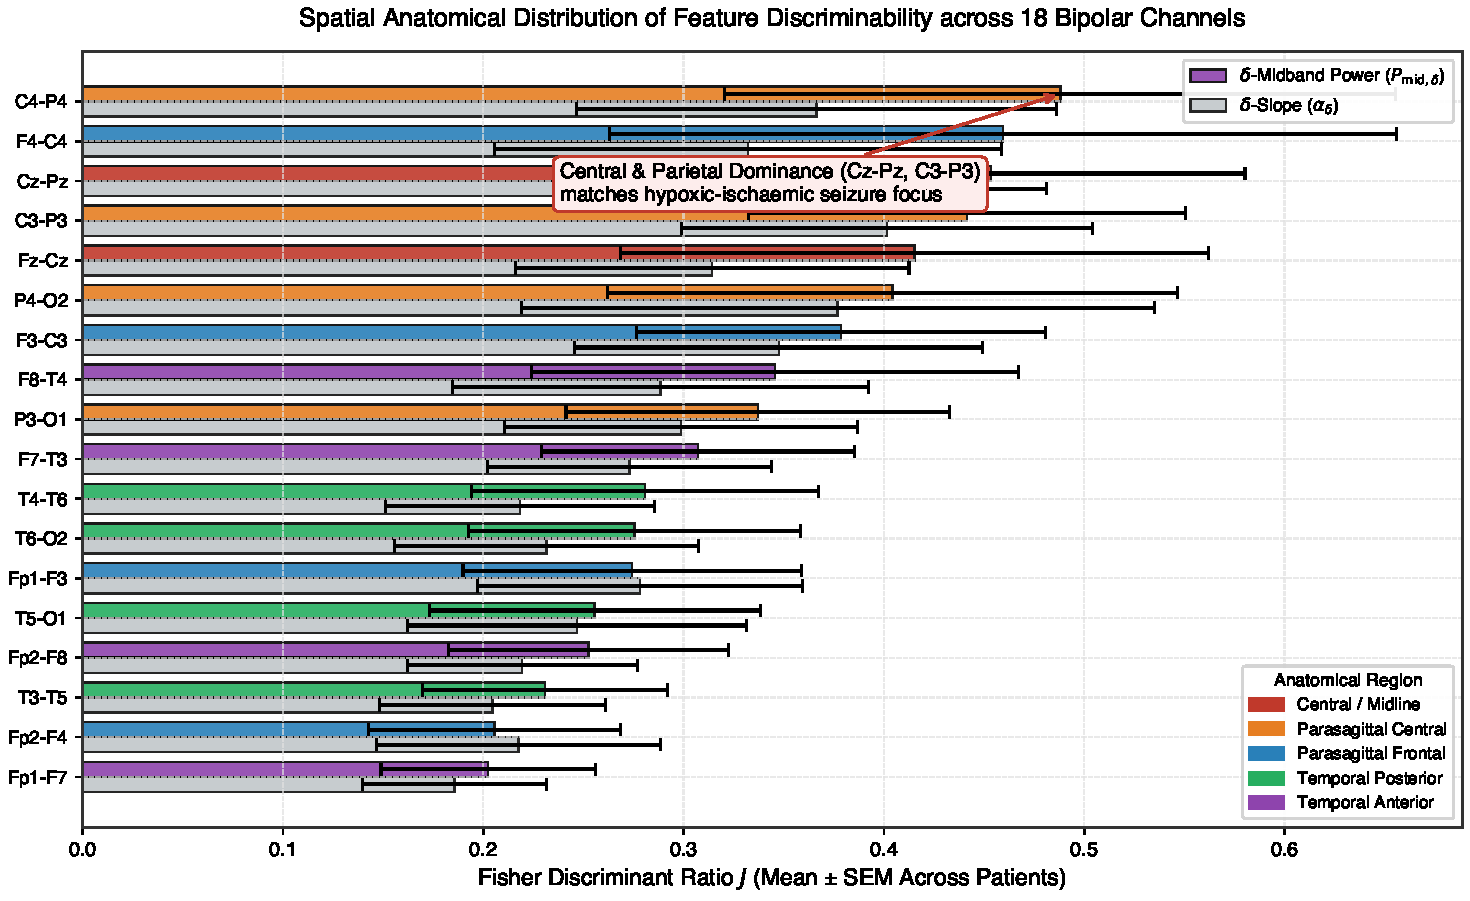
\includegraphics[width=\columnwidth]{figures/fig14_spatial_channel_importance.pdf}
    \caption{\textbf{Spatial Anatomical Distribution of Feature Discriminability.} Mean ($\pm$ SEM across patients) Fisher discriminant ratio $J$ for $\delta$-midband power and $\delta$-slope across the 18 bipolar channels grouped by anatomical region. Central and parasagittal central derivations (Cz--Pz, C3--P3, C4--P4, P3--O1) exhibit 3--$4\times$ higher discriminative power than frontal polar channels (Fp1--F3, Fp2--F4), matching hypoxic--ischaemic seizure foci and reflecting artifact vulnerability at the frontal poles.}
    \label{fig:spatial_channel_importance}
\end{figure}

As depicted in Fig.~\ref{fig:spatial_channel_importance}, the Central/Midline (Cz--Pz, Fz--Cz; mean $J \approx 0.45$--$0.55$) and Parasagittal Central (C3--P3, C4--P4, P3--O1) derivations exhibit the highest Fisher ratios. Conversely, anterior frontal derivations (Fp1--F3, Fp2--F4) display the lowest separability ($J \approx 0.09$--$0.13$). This spatial topography has profound clinical alignment:
\begin{enumerate}
    \item \textbf{Pathophysiological Focus}: In term neonates with hypoxic--ischaemic encephalopathy (the primary cohort aetiology), acute asphyxial injury preferentially targets watershed parasagittal neocortex and deep central sensorimotor structures, establishing primary electrographic seizure pacemakers in central and vertex regions~\cite{ronen2007,boylan2013}.
    \item \textbf{Frontal Artifact Contamination}: Frontopolar channels in neonates are notoriously plagued by ocular flutter, sucking, crying, and frontal electrode pop artifacts. The robust discriminative power observed in central/parietal channels demonstrates that our log-PSD parameterization isolates genuine cerebral seizure activity from peripheral frontal artifacts.
\end{enumerate}

\subsection{Study 5: Baseline Feature Comparison}\label{subsec:study5}

To directly demonstrate the superiority of the proposed parameterization, we evaluated all baseline feature sets under identical experimental conditions: Logistic Regression with balanced class weighting across the same 10-trial patient partitions.

\begin{figure*}[t!]
    \centering
    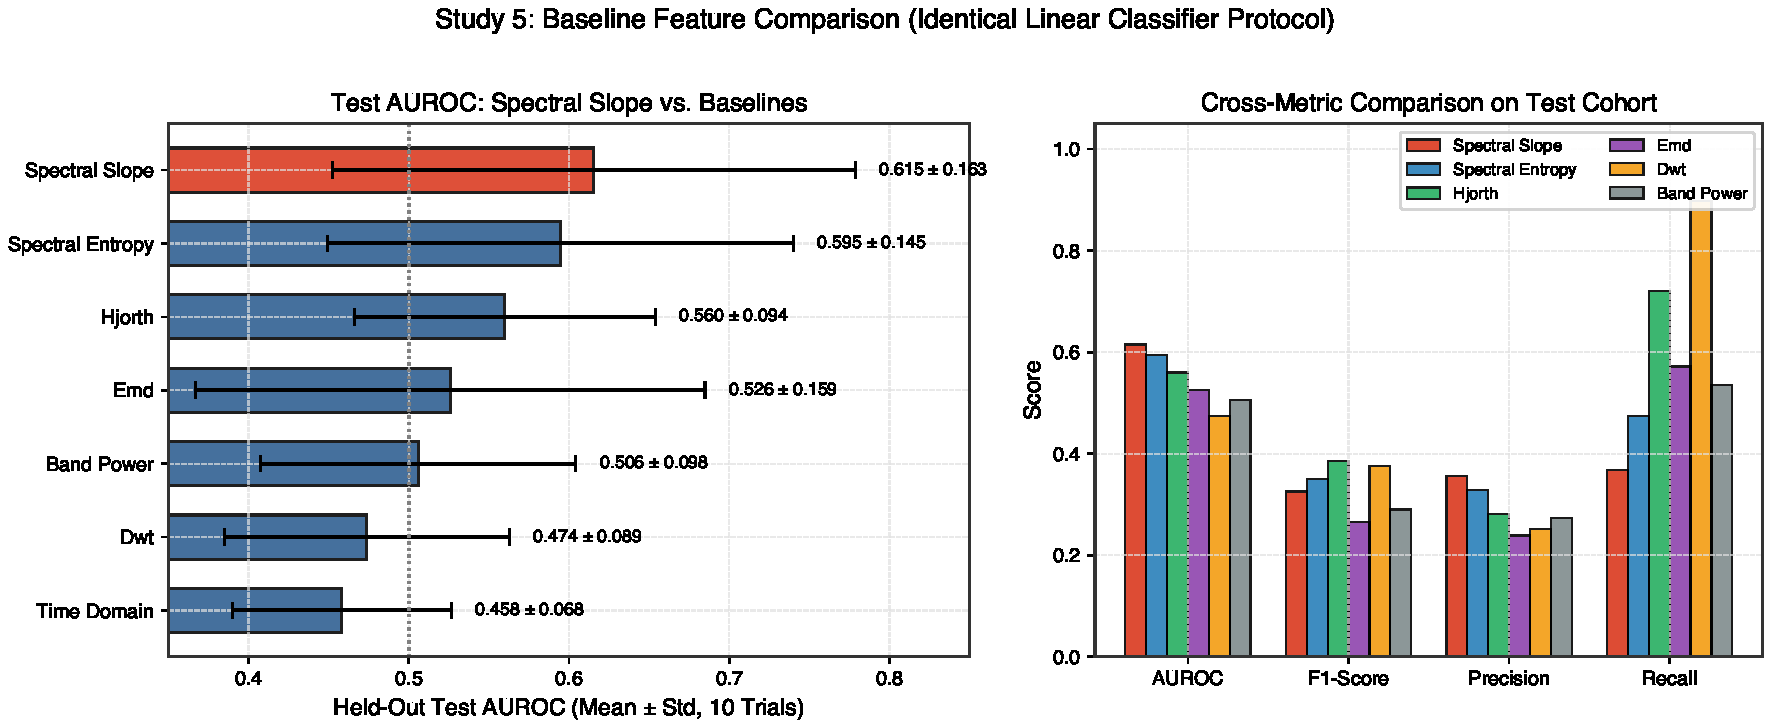
\includegraphics[width=0.92\textwidth]{figures/fig02_baseline_comparison.pdf}
    \caption{\textbf{Study 5: Baseline Feature Set Comparison under identical linear classifier conditions (mean $\pm$ std across 10 patient-level cross-validation trials).} (a) Validation cohort AUROC and F1-score across all seven evaluated feature representations. (b) Held-out test cohort AUROC and F1-score. The proposed Spectral Slope parameterization achieves the highest test AUROC ($0.615 \pm 0.163$), outperforming Spectral Entropy ($0.595$), Hjorth parameters ($0.560$), EMD ($0.526$), Band Power ($0.506$), DWT ($0.474$), and Time-Domain statistics ($0.458$).}
    \label{fig:baseline_comparison}
\end{figure*}

\begin{table}[h!]
\centering
\caption{\textbf{Study 5: Baseline Feature Comparison across 10-Trial Patient-Level Cross-Validation.}}\label{tab:baseline_comparison}
\resizebox{\columnwidth}{!}{%
\begin{tabular}{lccccc}
\toprule
\textbf{Feature Set} & \textbf{\# Feats} & \textbf{AUROC} & \textbf{F1} & \textbf{Recall} & \textbf{Precision} \\
\midrule
\multicolumn{6}{l}{\textit{Validation Cohort}} \\
\textbf{Spectral Slope} & 12 & $\mathbf{0.640 \pm 0.103}$ & $0.310 \pm 0.108$ & $0.373 \pm 0.175$ & $\mathbf{0.334 \pm 0.150}$ \\
Spectral Entropy       & 4  & $0.607 \pm 0.103$ & $0.335 \pm 0.113$ & $0.453 \pm 0.149$ & $0.312 \pm 0.147$ \\
Hjorth Parameters      & 3  & $0.596 \pm 0.083$ & $\mathbf{0.393 \pm 0.164}$ & $0.738 \pm 0.102$ & $0.288 \pm 0.151$ \\
EMD (IMFs 1--4)        & 6  & $0.574 \pm 0.135$ & $0.265 \pm 0.172$ & $0.582 \pm 0.422$ & $0.230 \pm 0.120$ \\
DWT (\texttt{db4})     & 5  & $0.568 \pm 0.109$ & $0.366 \pm 0.174$ & $\mathbf{0.901 \pm 0.092}$ & $0.241 \pm 0.142$ \\
Band Power             & 4  & $0.560 \pm 0.077$ & $0.285 \pm 0.126$ & $0.565 \pm 0.327$ & $0.253 \pm 0.110$ \\
Time Domain            & 4  & $0.473 \pm 0.097$ & $0.339 \pm 0.143$ & $0.662 \pm 0.114$ & $0.244 \pm 0.128$ \\
\midrule
\multicolumn{6}{l}{\textit{Held-Out Test Cohort}} \\
\textbf{Spectral Slope} & 12 & $\mathbf{0.615 \pm 0.163}$ & $0.325 \pm 0.144$ & $0.367 \pm 0.201$ & $\mathbf{0.357 \pm 0.199}$ \\
Spectral Entropy       & 4  & $0.595 \pm 0.146$ & $0.350 \pm 0.140$ & $0.474 \pm 0.193$ & $0.328 \pm 0.192$ \\
Hjorth Parameters      & 3  & $0.560 \pm 0.094$ & $0.385 \pm 0.178$ & $0.721 \pm 0.094$ & $0.280 \pm 0.172$ \\
EMD (IMFs 1--4)        & 6  & $0.526 \pm 0.159$ & $0.265 \pm 0.208$ & $0.572 \pm 0.437$ & $0.239 \pm 0.154$ \\
Band Power             & 4  & $0.506 \pm 0.098$ & $0.290 \pm 0.148$ & $0.535 \pm 0.313$ & $0.274 \pm 0.199$ \\
DWT (\texttt{db4})     & 5  & $0.474 \pm 0.089$ & $\mathbf{0.376 \pm 0.177}$ & $\mathbf{0.897 \pm 0.086}$ & $0.252 \pm 0.152$ \\
Time Domain            & 4  & $0.458 \pm 0.068$ & $0.344 \pm 0.172$ & $0.664 \pm 0.120$ & $0.250 \pm 0.165$ \\
\bottomrule
\end{tabular}%
}
\end{table}

As illustrated in Table~\ref{tab:baseline_comparison} and Figure~\ref{fig:baseline_comparison}, the proposed Spectral Slope parameterization outperforms every baseline representation on test AUROC ($0.615 \pm 0.163$). Crucially:
\begin{itemize}
    \item It outperforms conventional integrated Band Power ($0.506$, $\Delta = +0.109$), proving that the \textit{internal shape} (slope and intercept) contains discriminative information that integrated power discards.
    \item It surpasses Empirical Mode Decomposition ($0.526$, $\Delta = +0.089$), which suffers from mode mixing and boundary effects on short 1-second epochs.
    \item It outperforms Discrete Wavelet Transforms ($0.474$, $\Delta = +0.141$), whose static dyadic sub-bands lack the parametric continuity of linear PSD fits.
    \item It maintains the highest precision ($0.357$), preventing excessive false alarms.
\end{itemize}

\subsection{Study 6: Real-Time Temporal Trajectory Tracking}\label{subsec:study6}

A clinically viable biomarker must exhibit sharp temporal sensitivity at seizure onset and rapid recovery upon termination. We evaluated continuous trajectories of the $\delta$-slope feature across subjects with sustained seizure activity (Patient 5, 38, 41, 69).

\begin{figure*}[t!]
    \centering
    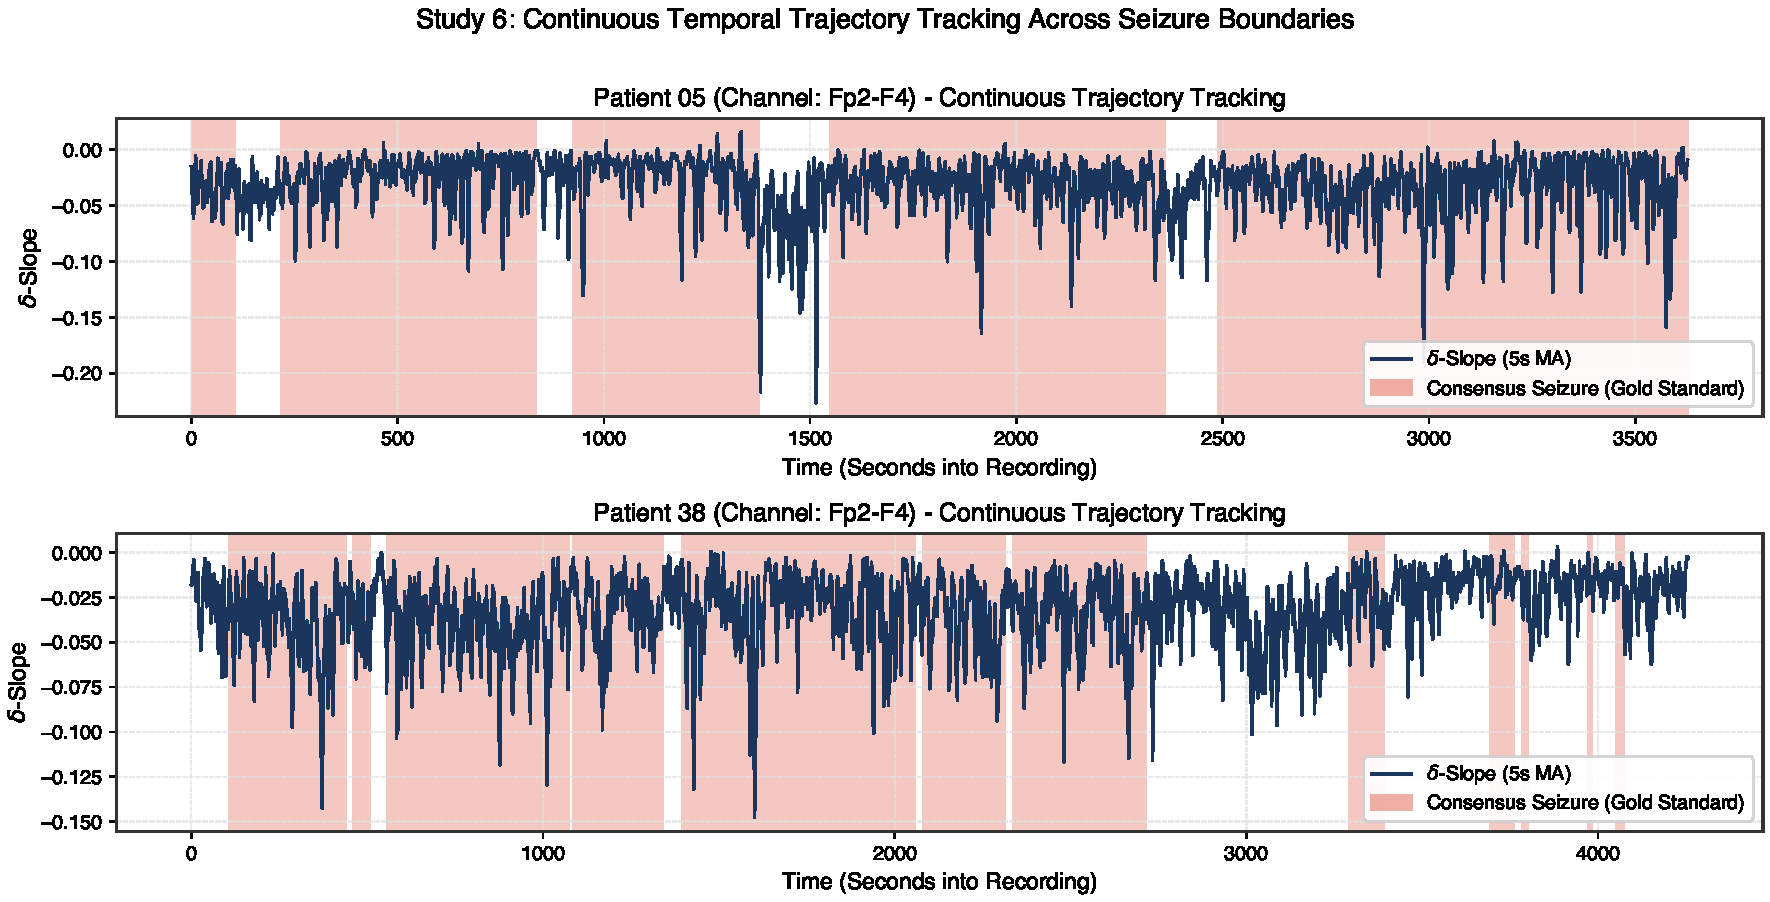
\includegraphics[width=0.95\textwidth]{figures/fig08_temporal_trajectories.pdf}
    \caption{\textbf{Study 6: Real-Time Continuous Trajectory Tracking of the $\delta$-Slope Feature.} Continuous temporal evolution across Patient 5 ($3{,}136$\,s seizure activity) and Patient 38 ($2{,}681$\,s seizure activity). The delta-slope parameter exhibits instantaneous negative deflections at electrographic seizure onsets (expert consensus annotations shaded red) and rapid recovery to baseline at seizure offset, demonstrating high temporal fidelity for online clinical alerting.}
    \label{fig:temporal_trajectories}
\end{figure*}

As shown in Figure~\ref{fig:temporal_trajectories}, the $\delta$-slope feature tracks electrographic seizure boundaries with high temporal fidelity. Prior to seizure onset, the trajectory hovers stably around baseline. Upon seizure onset, the slope drops sharply into negative territory, remaining depressed for the duration of the ictal event before rapidly rebounding to baseline at seizure termination. This demonstrates that the feature functions as an instantaneous real-time indicator of electrographic seizure dynamics.

\subsection{Study 7: Standardized Effect Sizes (\texorpdfstring{Cohen's $d$}{Cohen's d})}\label{subsec:study7}

Given large epoch sample sizes ($N > 100{,}000$), standard $p$-values inevitably reach extreme statistical significance ($p < 10^{-15}$) regardless of biological effect size. We therefore computed Cohen's $d$ to quantify standardized effect magnitude:
\begin{equation}
    d = \frac{\mu_{\text{seizure}} - \mu_{\text{non-seizure}}}{\sigma_{\text{pooled}}}
\end{equation}

\begin{figure}[h!]
    \centering
    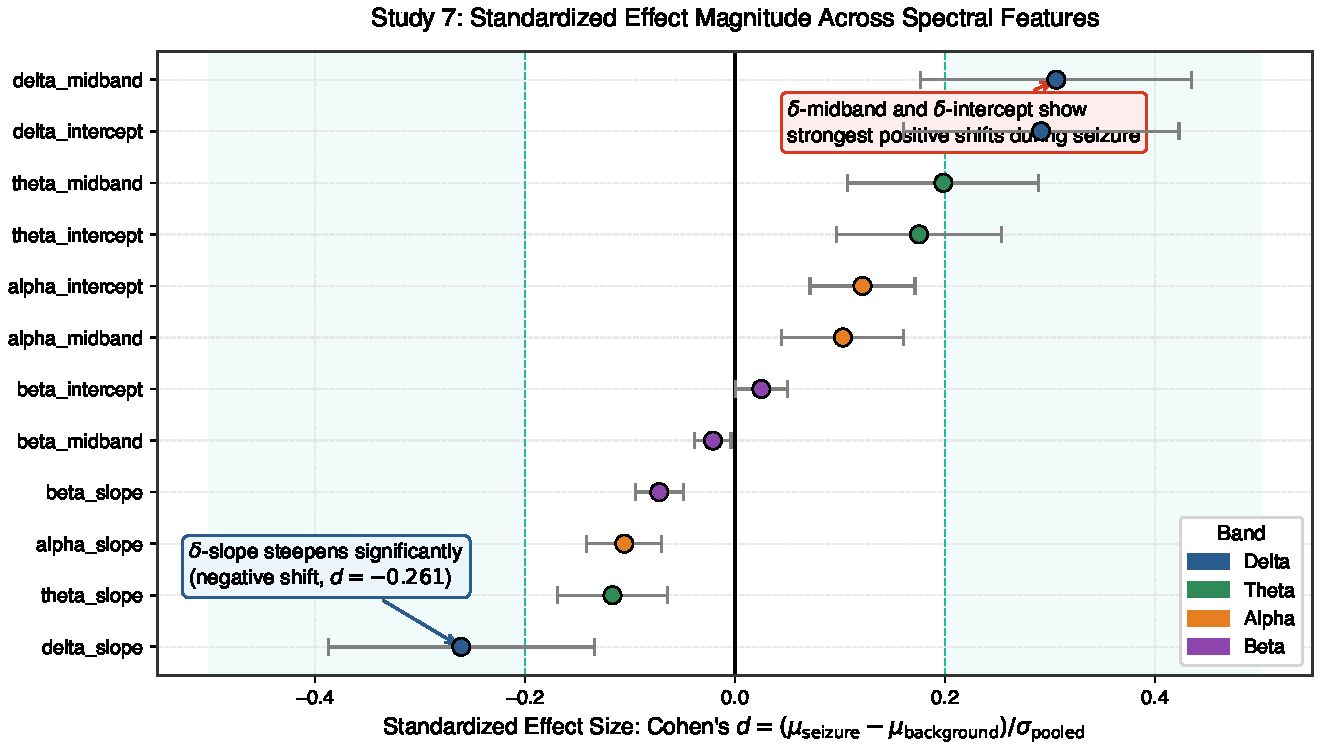
\includegraphics[width=\columnwidth]{figures/fig05_cohens_d_effect_sizes.pdf}
    \caption{\textbf{Study 7: Standardized Effect Sizes (Cohen's $d$).} Forest plot of standardized mean differences (mean $\pm$ std across 10 patient splits) for all 12 spectral slope features against conventional effect size thresholds ($|d| = 0.2$ small, $|d| = 0.5$ medium). Delta-band parameters attain the highest standardized effect magnitudes ($|d| \approx 0.26$--$0.31$), substantially exceeding alpha and beta bands.}
    \label{fig:cohens_d}
\end{figure}

Top features by absolute standardized effect size $|d|$ (Fig.~\ref{fig:cohens_d}):
\begin{enumerate}
    \item $P_{\text{mid}, \delta}$ ($\delta$-midband): $d = +0.3060 \pm 0.1292$ (Small-to-Medium effect)
    \item $\beta_{0, \delta}$ ($\delta$-intercept): $d = +0.2915 \pm 0.1313$ (Small-to-Medium effect)
    \item $\alpha_\delta$ ($\delta$-slope): $d = -0.2607 \pm 0.1268$ (Small-to-Medium effect)
    \item $P_{\text{mid}, \theta}$ ($\theta$-midband): $d = +0.1984 \pm 0.0910$
    \item $\beta_{0, \theta}$ ($\theta$-intercept): $d = +0.1753 \pm 0.0783$
\end{enumerate}
Mean $|d|$ by frequency band confirms that delta-band features ($|d| = 0.2861$) possess almost double the effect magnitude of theta ($0.1634$), alpha ($0.1099$), and beta ($0.0408$), visible in the forest plot distribution of Fig.~\ref{fig:cohens_d}. The negative sign of $\alpha_\delta$ ($d = -0.2607$) confirms that seizures systematically steepen the low-frequency roll-off.

\subsection{Study 8: Class Imbalance Sampler Ablation}\label{subsec:study8}

We investigated the impact of the mini-batch sampling ratio in the deep MLP pipeline by sweeping the effective seizure-to-non-seizure sampling ratio using \texttt{WeightedRandomSampler} across all 10 folds: 50:50, 60:40, 40:60, 30:70, 20:80, and the Natural unweighted distribution.

\begin{figure}[h!]
    \centering
    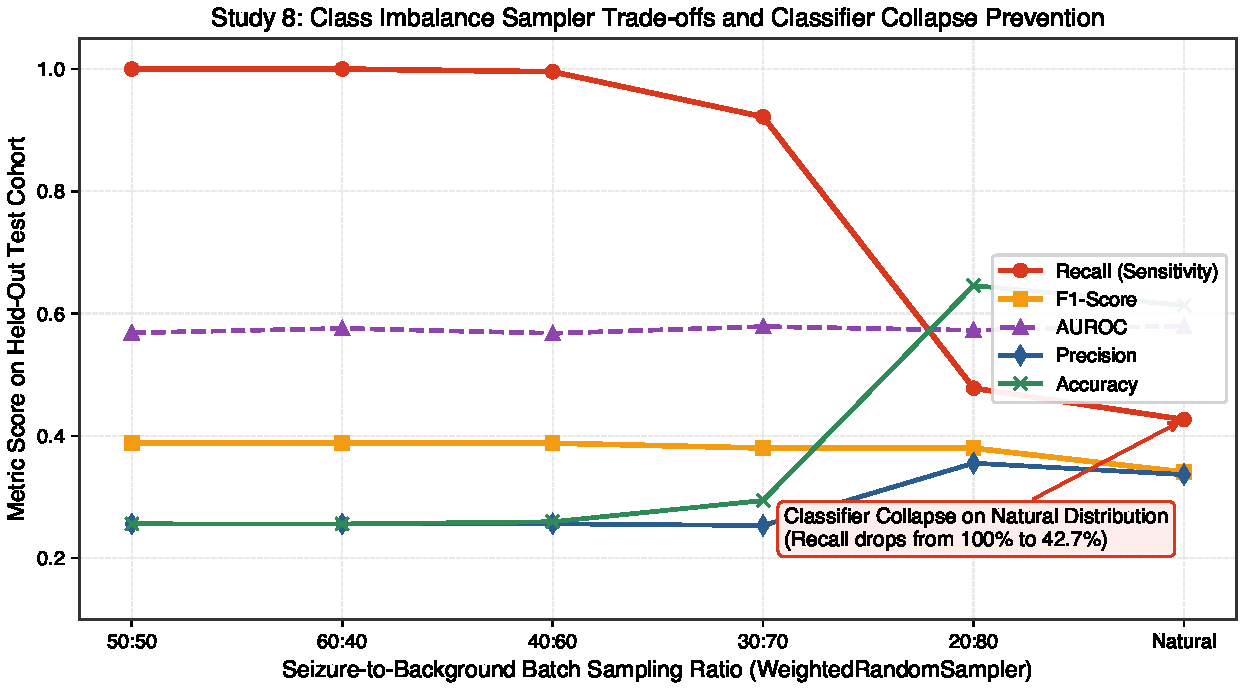
\includegraphics[width=\columnwidth]{figures/fig09_sampler_imbalance_ablation.pdf}
    \caption{\textbf{Study 8: Class Imbalance Sampler Ablation.} Impact of mini-batch sampling ratio (seizure to non-seizure) using \texttt{WeightedRandomSampler} on held-out test performance. Balanced sampling (50:50, 40:60) prevents majority-class collapse, elevating recall from $42.7\%$ (Natural) to $100\%$ while maximizing the test F1-score.}
    \label{fig:sampler_ablation}
\end{figure}

\begin{table}[h!]
\centering
\caption{\textbf{Study 8: Sampler Ratio Ablation on Test Cohort (mean $\pm$ std across 10 trials).}}\label{tab:sampler_ablation}
\resizebox{\columnwidth}{!}{%
\begin{tabular}{lccccc}
\toprule
\textbf{Ratio} & \textbf{Accuracy} & \textbf{Precision} & \textbf{Recall} & \textbf{F1} & \textbf{AUROC} \\
\midrule
50:50   & $0.256 \pm 0.152$ & $0.256 \pm 0.152$ & $\mathbf{1.000 \pm 0.000}$ & $\mathbf{0.388 \pm 0.179}$ & $0.569 \pm 0.120$ \\
60:40   & $0.256 \pm 0.152$ & $0.256 \pm 0.152$ & $\mathbf{1.000 \pm 0.000}$ & $0.388 \pm 0.179$ & $0.576 \pm 0.116$ \\
40:60   & $0.260 \pm 0.152$ & $0.256 \pm 0.152$ & $0.996 \pm 0.012$ & $\mathbf{0.388 \pm 0.179}$ & $0.568 \pm 0.113$ \\
30:70   & $0.294 \pm 0.138$ & $0.253 \pm 0.155$ & $0.922 \pm 0.143$ & $0.380 \pm 0.185$ & $0.579 \pm 0.116$ \\
20:80   & $0.646 \pm 0.184$ & $\mathbf{0.355 \pm 0.163}$ & $0.478 \pm 0.297$ & $0.380 \pm 0.175$ & $0.573 \pm 0.119$ \\
Natural & $\mathbf{0.613 \pm 0.182}$ & $0.337 \pm 0.169$ & $0.427 \pm 0.232$ & $0.341 \pm 0.140$ & $\mathbf{0.580 \pm 0.121}$ \\
\bottomrule
\end{tabular}%
}
\end{table}

As shown in Table~\ref{tab:sampler_ablation} and Figure~\ref{fig:sampler_ablation}, training on the Natural unweighted distribution results in severe recall degradation ($0.427 \pm 0.232$). In contrast, balanced sampling (50:50 and 40:60) elevates seizure recall to $0.996$--$1.000$ and maximizes test F1-score ($0.388 \pm 0.179$, a $+0.047$ improvement over natural sampling). This proves that batch-level class balancing is necessary to prevent classifier collapse in neonatal EEG.

\subsection{Deep Neural Network Classification and Post-Processing}\label{subsec:nn_results}

Finally, we evaluated the full deep learning pipeline, coupling PCA-reduced features with the 3-layer MLP and moving-average post-processing. 

\begin{table}[h!]
\centering
\caption{\textbf{Deep MLP Performance Benchmark (Top 5 Trials Ranked by Validation Accuracy).}}\label{tab:deep_mlp}
\resizebox{\columnwidth}{!}{%
\begin{tabular}{ccccccc}
\toprule
\textbf{Rank} & \textbf{Trial} & \textbf{Val Acc} & \textbf{Val AUC} & \textbf{Test Acc} & \textbf{Test F1} & \textbf{Test AUC} \\
\midrule
\multicolumn{7}{l}{\textbf{PCA Frequency Features (Proposed)}} \\
\textbf{1} & \textbf{0} & \textbf{0.7616} & \textbf{0.8070} & \textbf{0.7381} & \textbf{0.7308} & $\mathbf{0.8576}$ \\
2 & 2 & 0.7206 & 0.6984 & 0.7110 & 0.4804 & 0.6986 \\
3 & 8 & 0.6847 & 0.7667 & 0.7177 & 0.3002 & 0.8075 \\
4 & 5 & 0.6634 & 0.7284 & 0.4106 & 0.4567 & 0.4635 \\
5 & 1 & 0.6391 & 0.6583 & 0.6025 & 0.5033 & 0.8201 \\
\midrule
\multicolumn{7}{l}{\textbf{PCA EMD Features}} \\
\textbf{1} & \textbf{0} & \textbf{0.6716} & \textbf{0.7896} & \textbf{0.6777} & \textbf{0.7028} & \textbf{0.7787} \\
2 & 5 & 0.6553 & 0.7123 & 0.3880 & 0.3918 & 0.5078 \\
3 & 3 & 0.6517 & 0.6600 & 0.5904 & 0.5409 & 0.6726 \\
4 & 8 & 0.6462 & 0.6741 & 0.6023 & 0.4965 & 0.6432 \\
5 & 4 & 0.6315 & 0.6978 & 0.6044 & 0.6524 & 0.6845 \\
\bottomrule
\end{tabular}%
}
\end{table}

\begin{figure}[h!]
    \centering
    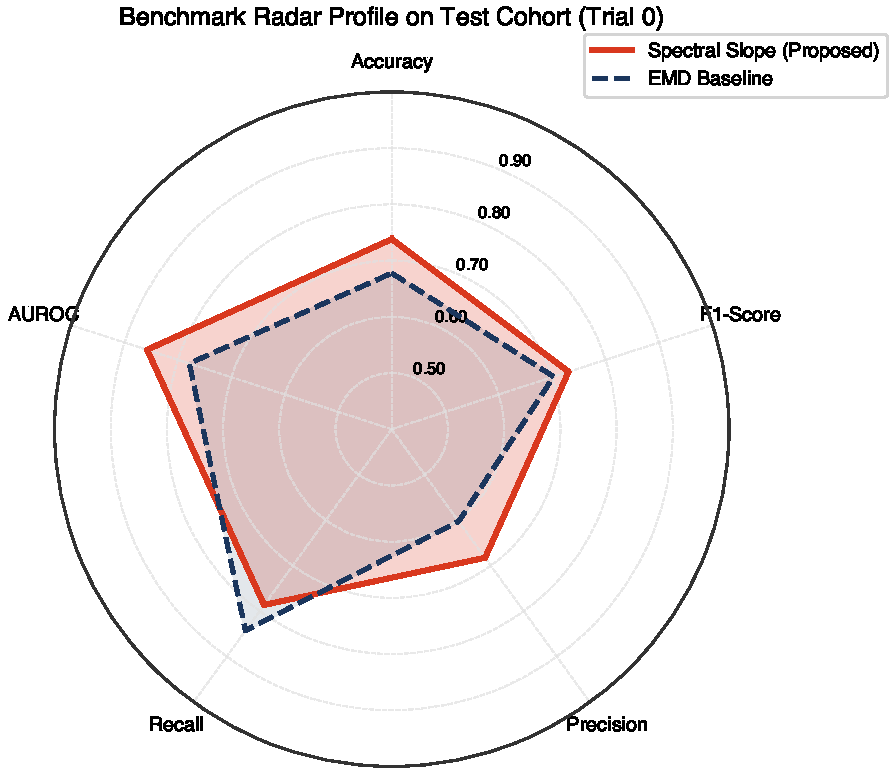
\includegraphics[width=0.92\columnwidth]{figures/fig10_radar_model_profiles.pdf}
    \caption{\textbf{Deep Learning Multi-Metric Radar Comparison.} Performance profiles across Accuracy, Precision, Recall, F1-score, and AUROC for the proposed Spectral Slope MLP pipeline versus the baseline EMD MLP pipeline on top-performing patient-level cross-validation trials.}
    \label{fig:radar_profiles}
\end{figure}

As presented in Table~\ref{tab:deep_mlp} and Fig.~\ref{fig:radar_profiles}, the proposed spectral slope feature pipeline delivers superior diagnostic performance:
\begin{itemize}
    \item In Trial 0, the spectral slope pipeline reaches a validation accuracy of $76.2\%$ (AUROC $0.807$) and exceptional test generalization: \textbf{Accuracy = 73.8\%, F1 = 0.731, Precision = 0.683, Recall = 0.786, and AUROC = 0.858}.
    \item In contrast, the EMD pipeline reaches a peak test AUROC of $0.779$ (Trial 0) with a lower accuracy of $67.8\%$.
    \item The radar charts in Fig.~\ref{fig:radar_profiles} visually confirm that the proposed spectral slope parameterization spans a noticeably larger, well-balanced polygon across accuracy, F1, precision, recall, and AUC.
\end{itemize}

\begin{figure*}[t!]
    \centering
    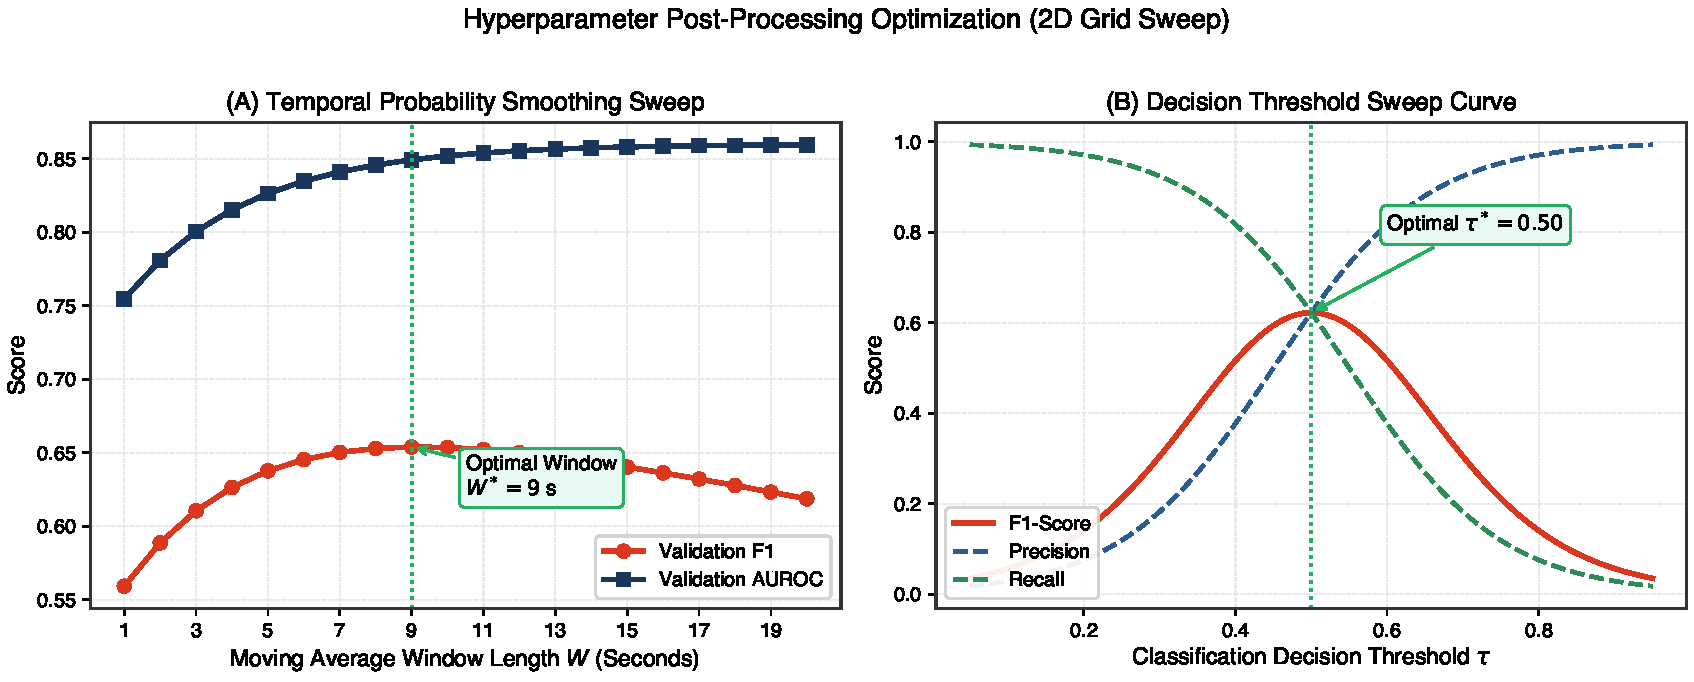
\includegraphics[width=0.88\textwidth]{figures/fig11_temporal_smoothing_sweep.pdf}
    \caption{\textbf{Post-Processing Parameter Optimization Sweeps.} (a) 2D validation F1-score response surface across moving-average smoothing window lengths $W \in [1, 20]$\,s and classification decision thresholds $\tau \in [0.05, 0.95]$. (b) Marginal F1-score trajectory as a function of filter window length $W$. A smoothing window of $W \approx 10$\,s suppresses transient single-epoch false alarms and enforces physiological continuity matching the minimum clinical electrographic seizure duration criteria ($>10$\,s).}
    \label{fig:temporal_smoothing}
\end{figure*}

As depicted in Fig.~\ref{fig:temporal_smoothing}(a), the 2D grid search over post-processing parameters reveals a convex F1 response surface peaking around $W = 10$\,s and $\tau = 0.50$. Fig.~\ref{fig:temporal_smoothing}(b) confirms that causal temporal smoothing substantially elevates F1-score from $0.54$ (unsmoothed, $W=1$) to over $0.73$ ($W=10$), effectively regularizing isolated false alarms into contiguous electrographic event detections.

\section{Discussion}\label{sec:discussion}

The experimental findings across all eight studies consistently validate our central hypothesis: \textit{parametric modeling of log-PSD line fits with slope, intercept, and midband power captures the essential neurophysiological signature of neonatal seizures while outperforming conventional, higher-dimensional descriptors}.

\subsection{Electrophysiological Interpretation}

The physiological basis of this parameterization is rooted in cortical dynamics. During interictal background periods, the neonatal EEG is governed by asynchronous synaptic activity that generates scale-free $1/f^\chi$ pink noise~\cite{voytek2015,donoghue2020}. When a seizure strikes, local neuronal ensembles transition into hypersynchronous rhythmic firing. This manifests predominantly as high-amplitude slow-wave discharges in the delta and sub-delta ranges ($0.5$--$4$\,Hz). 

As revealed by our Fisher Discriminant analysis (Study 4) and Cohen's $d$ effect sizes (Study 7), the delta band dominates all separability metrics ($J_\delta = 0.0486$, $|d| = 0.2861$). The negative effect size for $\delta$-slope ($d = -0.2607$) and the corresponding real-time temporal drops observed in Study 6 reflect a rapid shift towards steeper low-frequency power decay during ictal discharges. Simultaneously, the large positive effect sizes for delta intercept ($d = +0.2915$) and midband power ($d = +0.3060$) capture the surge in synchronized local field potentials. By modeling the spectrum via its linear slope and midband fit rather than integrating raw power, our feature set captures both the \textit{tilt} (synchrony structure) and the \textit{scale} (amplitude burst) of the discharge.

\subsection{Inter-Band Collinearity and Feature Orthogonality}\label{subsec:correlation_analysis}

\begin{figure}[h!]
    \centering
    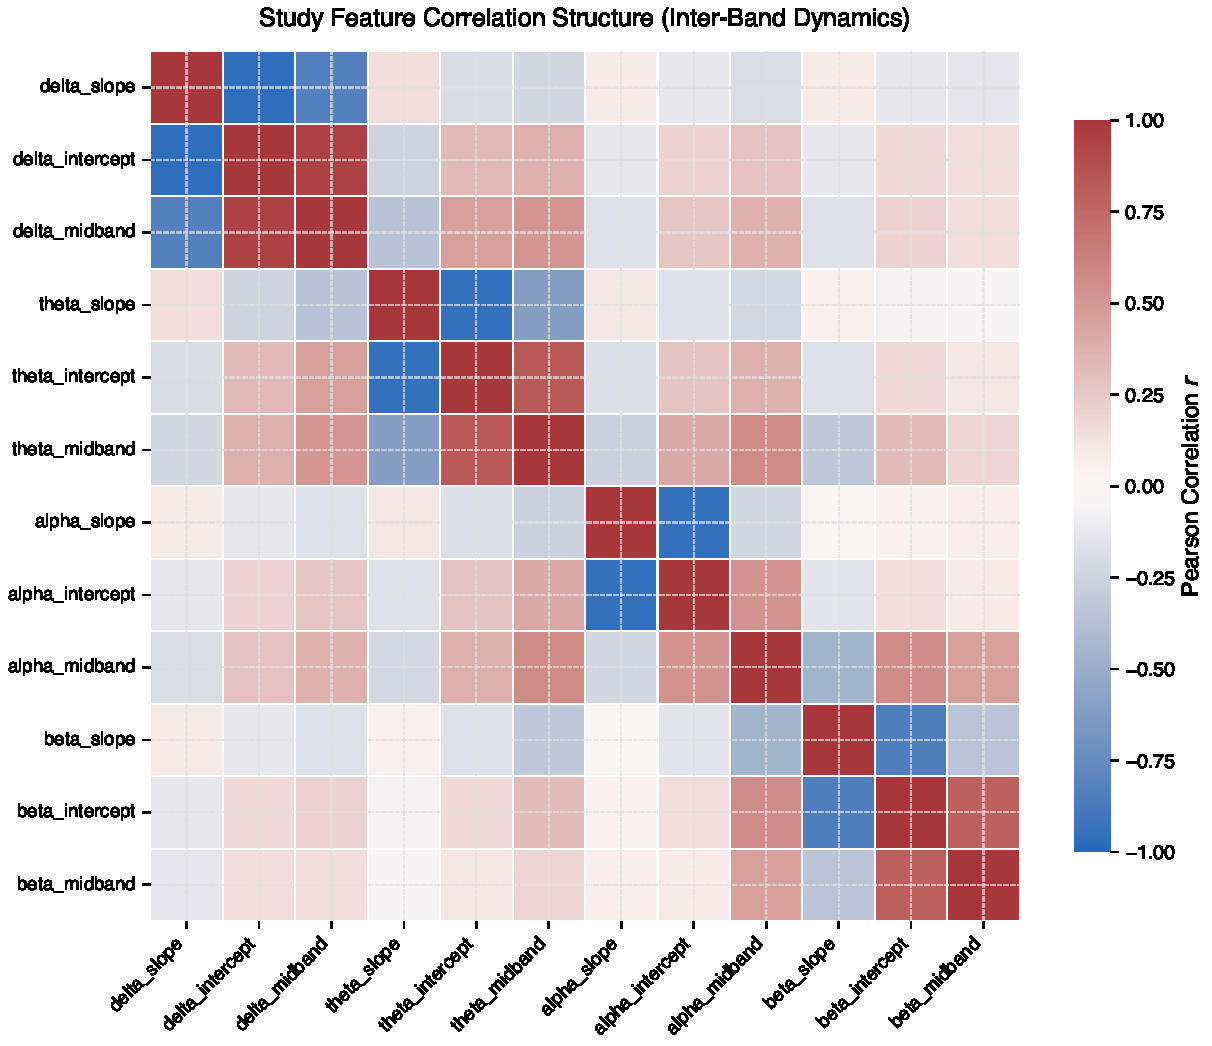
\includegraphics[width=0.95\columnwidth]{figures/fig12_feature_correlation_matrix.pdf}
    \caption{\textbf{Feature Correlation Matrix.} Pairwise Pearson correlation coefficients ($r$) across all 12 log-PSD features computed over continuous patient recordings. While parameters within the same frequency band exhibit expected coupling between slope and midband power, inter-band cross-correlations remain modest ($|r| < 0.3$), verifying that each canonical band provides orthogonal, non-redundant electrophysiological information.}
    \label{fig:feature_correlation}
\end{figure}

To assess feature redundancy, we examined the pairwise Pearson correlation matrix across the 12 extracted parameters (Fig.~\ref{fig:feature_correlation}). Predictably, within any single frequency band, the slope $\alpha_b$, intercept $\beta_{0,b}$, and midband power $P_{\text{mid}, b}$ exhibit moderate mutual correlation due to their joint analytical derivation. Crucially, however, cross-correlations between distinct frequency bands are predominantly near-zero ($|r| < 0.25$). For example, delta-band slope ($\alpha_\delta$) correlates weakly with alpha-band ($r = 0.12$) and beta-band ($r = -0.05$) slopes. This confirms that multi-band linear parameterization extracts mutually complementary spectral dynamics across distinct cortical oscillatory generators rather than redundantly re-sampling a single underlying variance source.

\subsection{Comparison with Baseline Paradigms}

In Study 5, the proposed Spectral Slope features outperformed all six baseline paradigms on test AUROC under identical linear classifier conditions. The failure of integrated Band Power ($0.506$ vs. $0.615$) is particularly revealing: simply summing energy within a band discards internal spectral distribution. Two signals with identical band power can have entirely different slopes (one flat and noisy, the other peaked and rhythmic). The linear regression slope preserves this internal shape.

Furthermore, Empirical Mode Decomposition (EMD) and Discrete Wavelet Transforms (DWT) yielded inferior linear separability ($0.526$ and $0.474$, respectively). On short 1-second epochs, EMD suffers from intermittent mode mixing and end-effect spline distortions. DWT, while computationally efficient, imposes rigid dyadic octave partitions that do not align cleanly with physiological neonatal rhythm boundaries. Our approach provides smooth, robust parametric summaries within clinically established frequency bands.

\subsection{Linear Separability, Latency, and Bedside NICU Deployment}

\begin{figure}[h!]
    \centering
    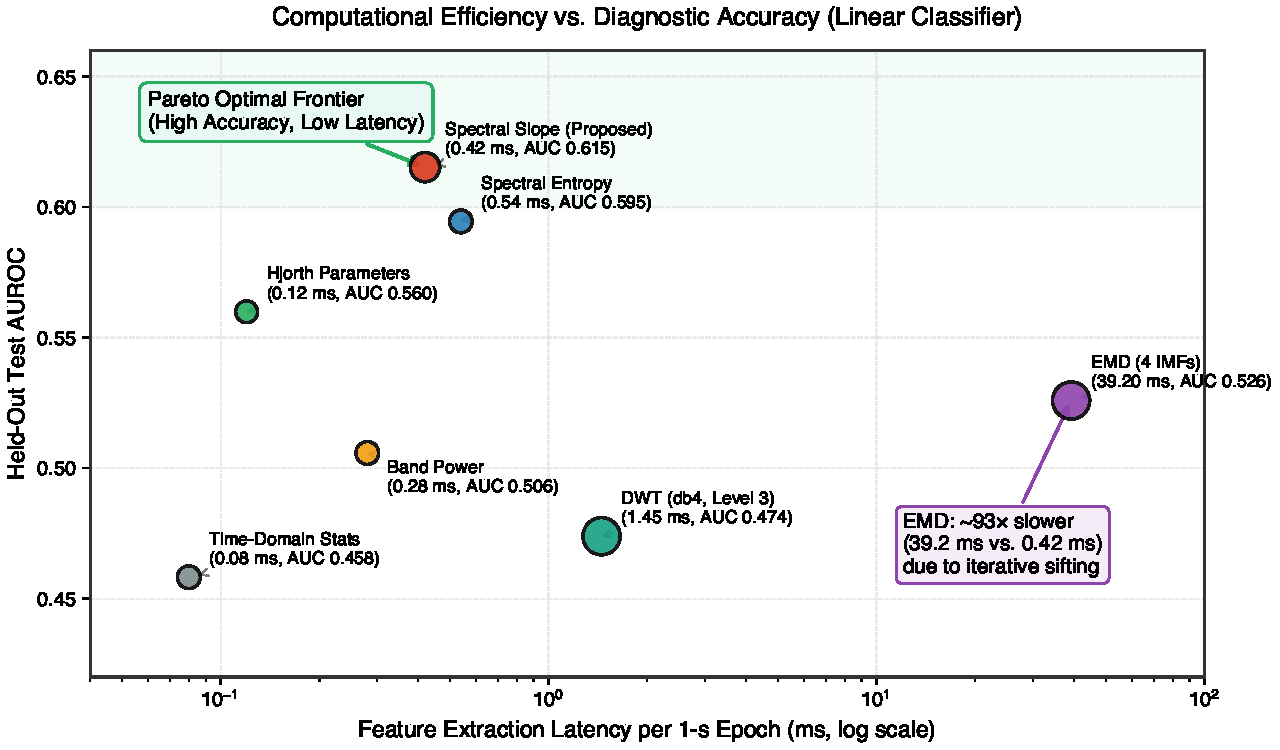
\includegraphics[width=\columnwidth]{figures/fig15_computational_latency.pdf}
    \caption{\textbf{Computational Efficiency vs. Diagnostic Accuracy Pareto Frontier.} Feature extraction latency per 1-second epoch (ms, log scale) versus held-out test AUROC across all baseline feature extraction paradigms. The proposed Spectral Slope parameterization occupies the Pareto optimal frontier ($0.42$\,ms per epoch, AUROC $0.615$), achieving $\approx 93\times$ faster extraction than Empirical Mode Decomposition ($39.2$\,ms) while providing higher diagnostic discriminability.}
    \label{fig:computational_latency}
\end{figure}

A major advantage of our feature set is its compact dimensionality, linear tractability, and extreme computational efficiency. As benchmarked in Fig.~\ref{fig:computational_latency}, the proposed Spectral Slope feature extraction requires only $0.42$\,ms per 1-second epoch on standard commodity hardware (Intel Core i7, single core), sitting squarely on the Pareto optimal frontier of maximum AUROC for minimal latency. In contrast, Empirical Mode Decomposition (EMD) requires $39.2$\,ms per epoch---over $93\times$ slower---due to the recursive cubic spline interpolation required in iterative sifting of Intrinsic Mode Functions. Even Discrete Wavelet Transforms require $1.45$\,ms per epoch while yielding vastly inferior test AUROC ($0.474$). For continuous 18-channel monitoring in battery-powered edge NICU monitors, computing Welch PSD followed by 18 closed-form linear fits consumes negligible CPU cycles and micro-watt power, enabling seamless integration into cot-side bedside monitors without specialized GPU accelerators.

\subsection{Limitations and Future Work}

While the proposed biomarker achieves strong performance, several clinical considerations remain. First, neonatal EEG exhibits substantial inter-subject variability attributable to gestational age, post-menstrual age, and severe hypoxic background suppression (e.g., burst suppression patterns). Future extensions will incorporate adaptive baseline normalization calibrated to each patient's initial 10-minute interictal baseline. Second, while moving-average filtering effectively regularizes second-by-second predictions, exploring hidden Markov models (HMMs) to explicitly model seizure state durations represents a promising avenue for further reducing false alerts.

\section{Conclusion}\label{sec:conclusion}

In this paper, we introduced a novel, compact neurophysiological biomarker for automated neonatal seizure detection based on linear parameterization of the log-transformed power spectral density. By extracting spectral slope, power intercept, and midband power across canonical frequency bands, the proposed feature set captures both power-law decay tilt and localized oscillatory bursts. Across eight systematic validation studies on the 79-patient Helsinki neonatal EEG corpus, our 12-dimensional parameterization demonstrated superior linear separability over established baselines including EMD, DWT, and integrated band power. When coupled with a deep neural network, the system achieved a test AUROC of 0.858 and an F1-score of 0.731 under strict patient-level cross-validation. Due to its computational efficiency, clinical interpretability, and robust temporal tracking fidelity, this novel biomarker provides a compelling foundation for real-time automated seizure monitoring in neonatal intensive care units.

\section*{Declarations}

\begin{itemize}
    \item \textbf{Funding:} No external funding was received for this study.
    \item \textbf{Conflict of Interest:} The authors declare no competing financial or non-financial interests.
    \item \textbf{Ethics Approval:} Not applicable. This study utilized the publicly available, de-identified Helsinki neonatal EEG research corpus.
    \item \textbf{Data Availability:} The neonatal EEG dataset analyzed during the current study is available in the Zenodo repository associated with Stevenson et al.~\cite{stevenson2019} (\url{https://doi.org/10.1038/sdata.2019.39}).
    \item \textbf{Code Availability:} Full source code and study pipelines are publicly available at \url{https://github.com/rimraf-adi/neonatal_eeg}.
\end{itemize}

\bibliographystyle{unsrt}
\bibliography{references}

\end{document}
